\documentclass{scrartcl}
\usepackage{color}
\usepackage{url}
\usepackage{cite}
\usepackage{eucal}
\usepackage{fancybox}
\usepackage{amsmath}
\usepackage{epsfig}
\usepackage{amssymb}
\usepackage{amsfonts}
\usepackage{hyperref}
\usepackage{listings}
\usepackage{caption,subcaption}
%
\newcommand{\TODO}[1]{\textcolor{red}{\boxed{\mathbf{TODO }} {\textit{#1}} }}
\newcommand{\REMARK}[1]{\textcolor{blue}{\boxed{\mathbf{Remark }} {\textit{#1}} }}
\newcommand{\todo}{\TODO}
\newcommand{\remark}{\REMARK}
\newcommand{\email}[1]{\texttt{#1}}
%
\begin{document}

\title{R-Trees - A Dynamic Index Structure for Spatial Searching}
\subtitle{CS 764 - Spring 2013 - Repeatability Project}

\author{
Aaron Gorenstein\\
	\email{agorenst@cs.wisc.edu}
\and
Rebecca Lam\\
	\email{rjlam@cs.wisc.edu}
\and
Cathrin Weiss\\
	\email{cweiss@cs.wisc.edu}       
}

\date{\today}

\maketitle

%====== INTRODUCTION =======================
\section{Introduction}
\label{sec:intro}
In \cite{DBLP:conf/sigmod/Guttman84}, Guttman proposes the R-Tree, an index structure for performing range queries on spatial data efficiently. The paper gives detailed descriptions of structure layout and algorithms needed for inserting, deleting, and searching data. 

In this report we present results and discussion of similar experiments run on our implementation of the R-Tree structure and compare experimental results to Guttman's original results.  

%====== EXPERIMENTS ==================
\section{Experiments}
\label{sec:experiments}
The experiments in~\cite{DBLP:conf/sigmod/Guttman84} were performed to demonstrate practicality of 
the index structure. In modern papers rather uncommon, the experiments do not compare the structure to 
previous structures for the same or similar purpose. Instead, two node splitting algorithms are proposed, 
one with quadratic, another with linear runtime, and compared to each other as well as a baseline 
algorithm with exponential runtime (the exhaustive algorithm). Experiments are performed on a defined data set. 

``Practicality'' as demonstrated in the original paper can be phrased out as the following hypotheses: 
\subsection{Hypotheses}
\paragraph{Hypothesis 1}
The linear algorithm outperforms quadratic and exhaustive algorithms for insert and delete.

\paragraph{Hypothesis 2}
More strict node-fill criteria increase insert performance, but decrease delete performance.

\paragraph{Hypothesis 3}
Search performance (CPU and number of pages touched) is insensitive to the choice of the node-split algorithm .

\paragraph{Hypothesis 4}
More strict node-fill criteria produce smaller indices.

\paragraph{Hypothesis 5}
Insert and delete operation cost increases proportionally with tree height but stays mostly constant for varying tree width.

\paragraph{Hypothesis 6}
Search cost per qualifying record decreases as the number of data records increases.

\paragraph{Hypothesis 7}
Since all data is stored in leaf nodes, space consumption increases linearly with the number of data entries. 

\subsection{Proxies and expected outcomes}
Fast forward almost 30 years later, we reimplemented the R-Tree structure in C++ compiled in 32 bit mode with optimization turned off. Some implementation overhead may be created by using STL vectors for a node's entry list, as well as for any further entry list management (node splits, for example).

As we do not have the original data available and to eliminate data bias, we ran experiments on two different data sets: First, on a randomly generated data set, which has positive integer values for $x$ and $y$ such that $10 < x_{\mathrm{min}} < x_{\mathrm{max}} < 1000$ and  $5 < y_{\mathrm{min}} < y_{\mathrm{max}} < 3000$. This data set contains many large, overlapping rectangles. A real world data example is our second data set taken from~\cite{Online:usppdata}, which consists of the points of populated places in the USA. The entire data set contains 15206 entries. This data has no overlapping records, but is widely distributed. We randomly sampled 1057 for the experiments for experiments relating to hypothesis 1-4, and between 1000 and 5000 for the rest of the experiments. Search rectangles resulting in 4-6\% of the data returned were randomly generated. For the delete process, we again randomized the order of entries from the initial data set and performed the deletes. In general we expect CPU times to be orders of magnitudes faster, i.e. expect to see microseconds per operation, or nanoseconds per qualifying search record. Visualizations of the data sets and the data sets overlaid by the set of search rectangles are shown in figures~\ref{fig:rdata}-\ref{fig:usdataSearch}.

Each described experiment was run ten times and the results averaged to eliminate system noise.

\begin{figure}
\centering
\begin{minipage}{0.49\textwidth}
\centering
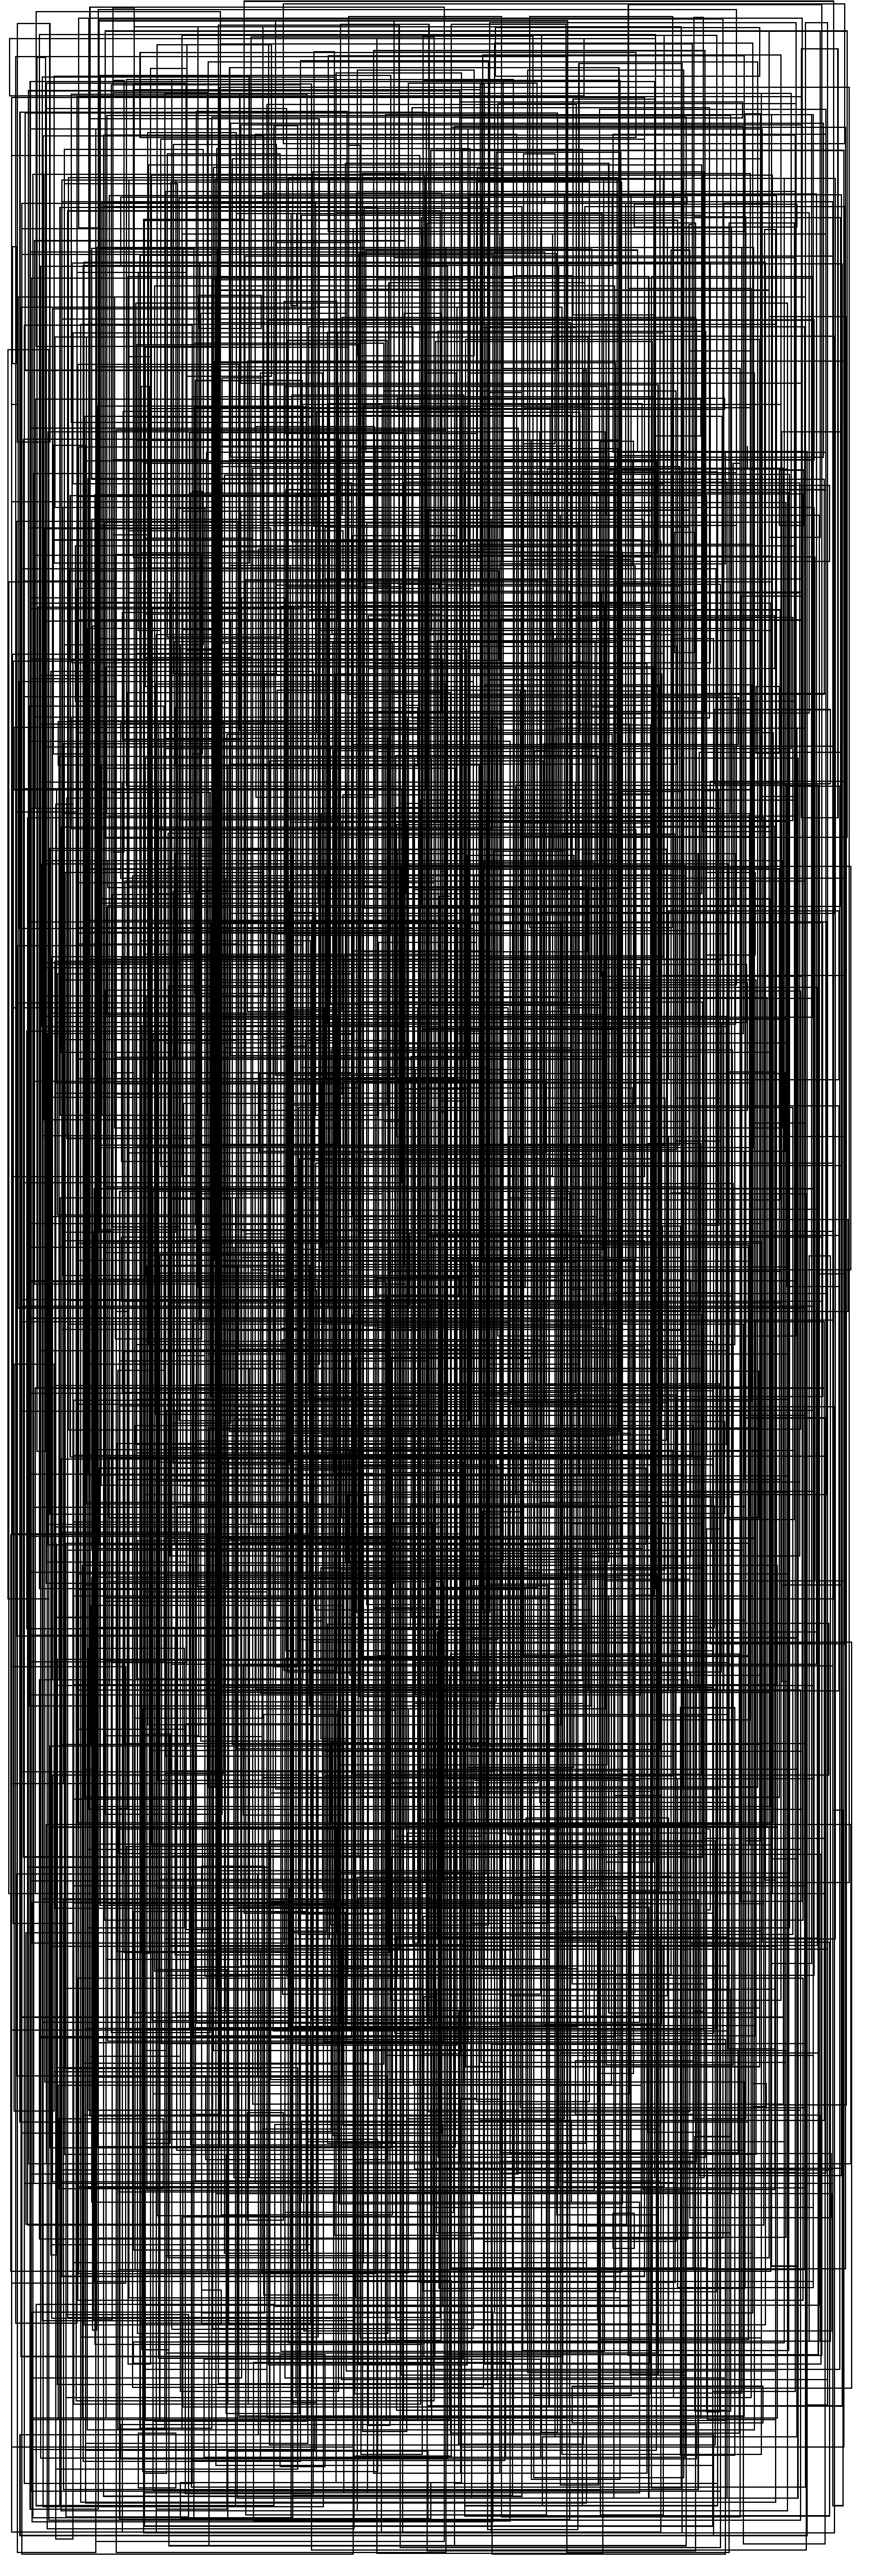
\includegraphics[width=.3\textwidth]{fig/randomData.pdf}
\caption{Random rectangle data - 1k rectangles}
\label{fig:rdata}
\end{minipage}
\begin{minipage}{0.49\textwidth}
\centering
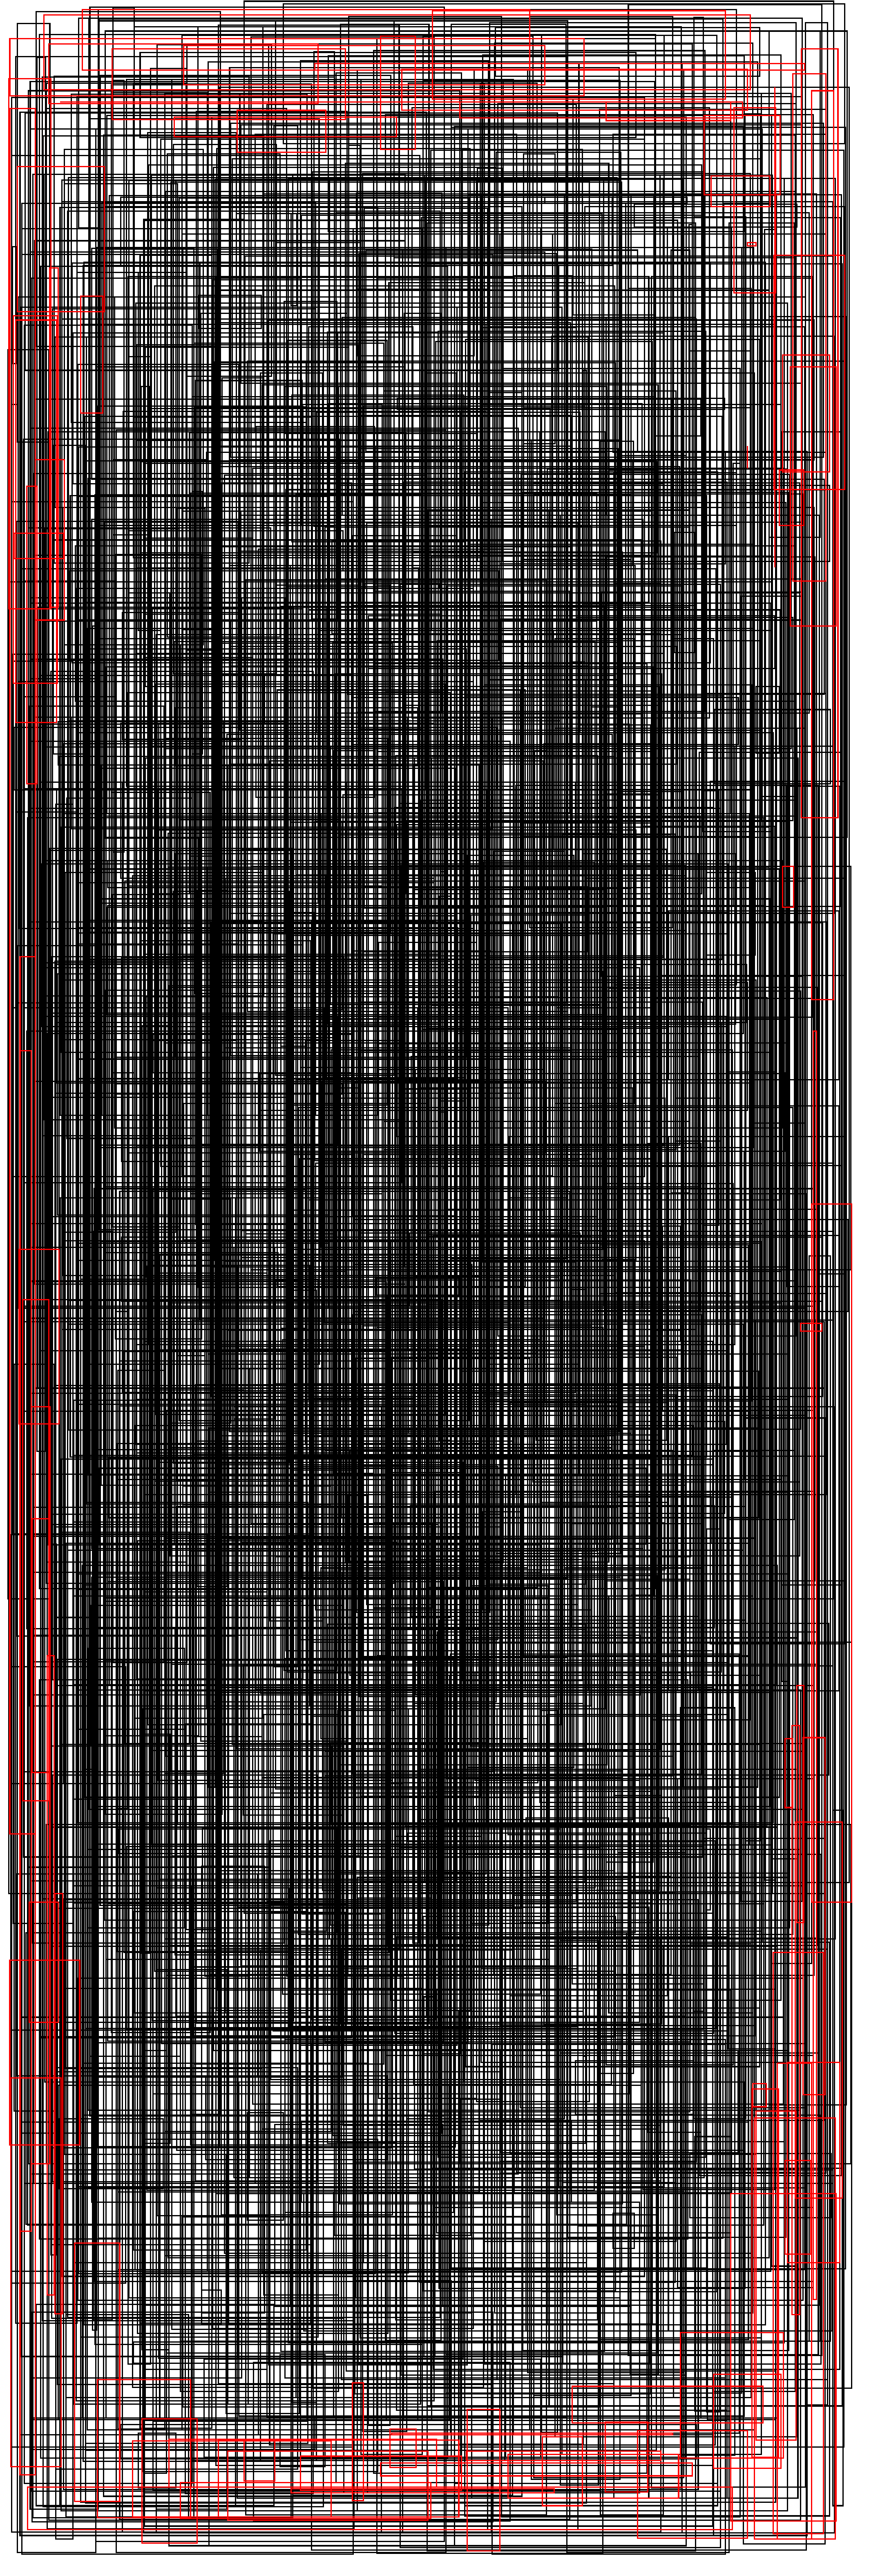
\includegraphics[width=.3\textwidth]{fig/randomDataSearch.pdf}
\caption{Random rectangle data - 1k rectangles - Search overlay}
\label{fig:rdataSearch}
\end{minipage}
\end{figure}
\begin{figure}
\centering
\begin{minipage}{\textwidth}
\centering
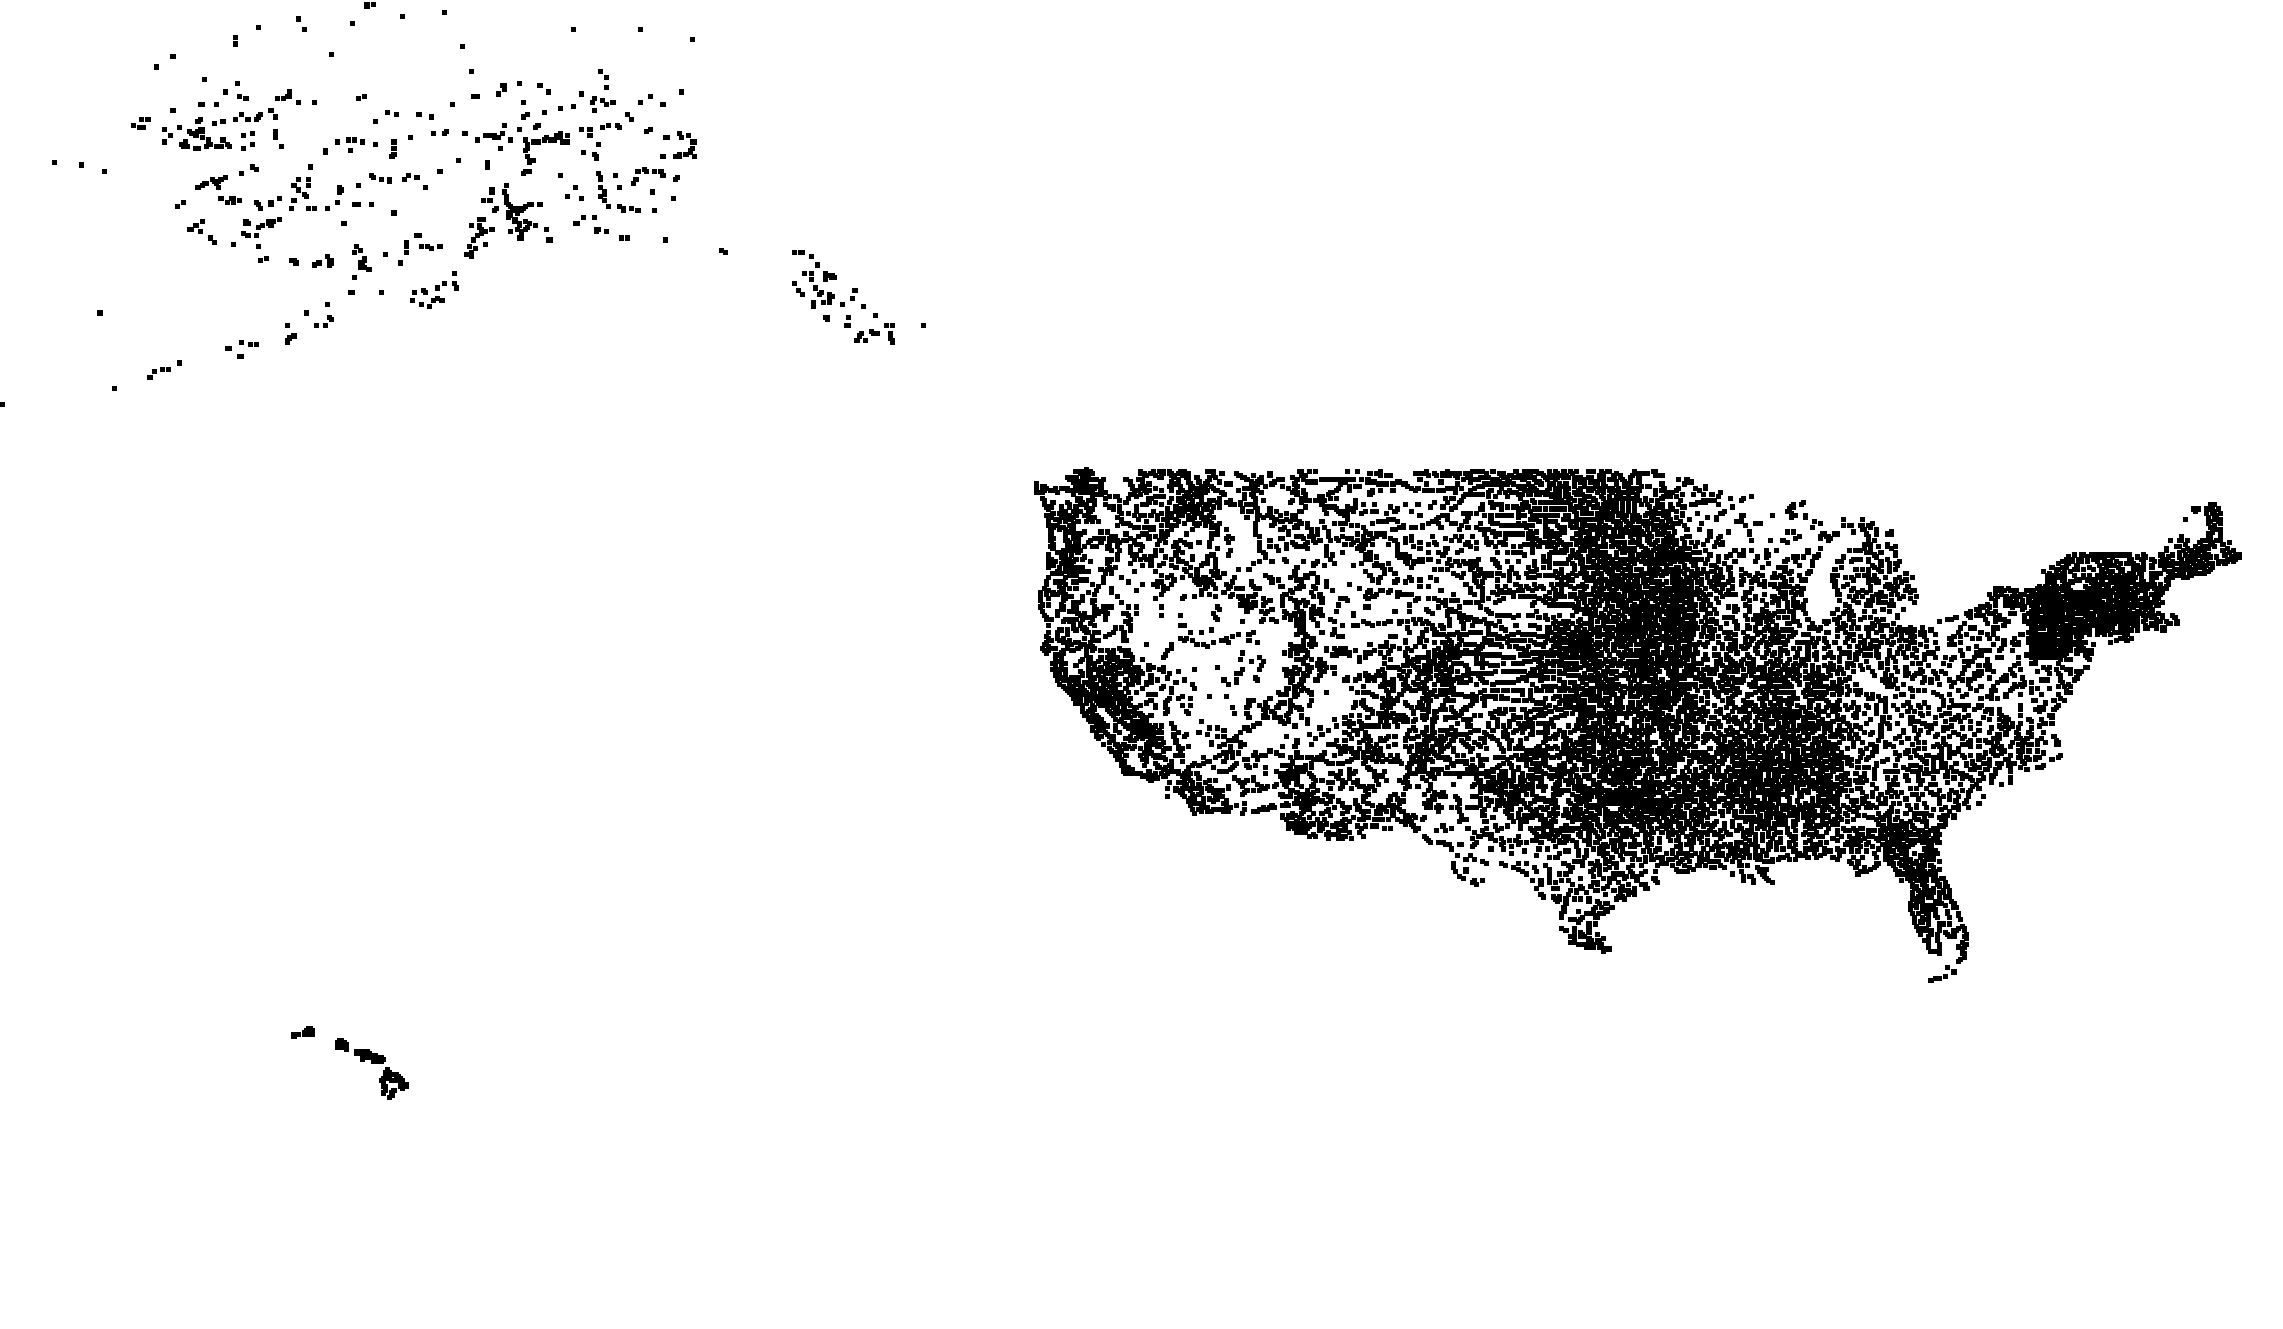
\includegraphics[width=.7\textwidth]{fig/usppp.pdf}
\caption{US points of populated places}
\label{fig:usdata}
\end{minipage}
\end{figure}
\begin{figure}
\centering
\begin{minipage}{0.49\textwidth}
\centering
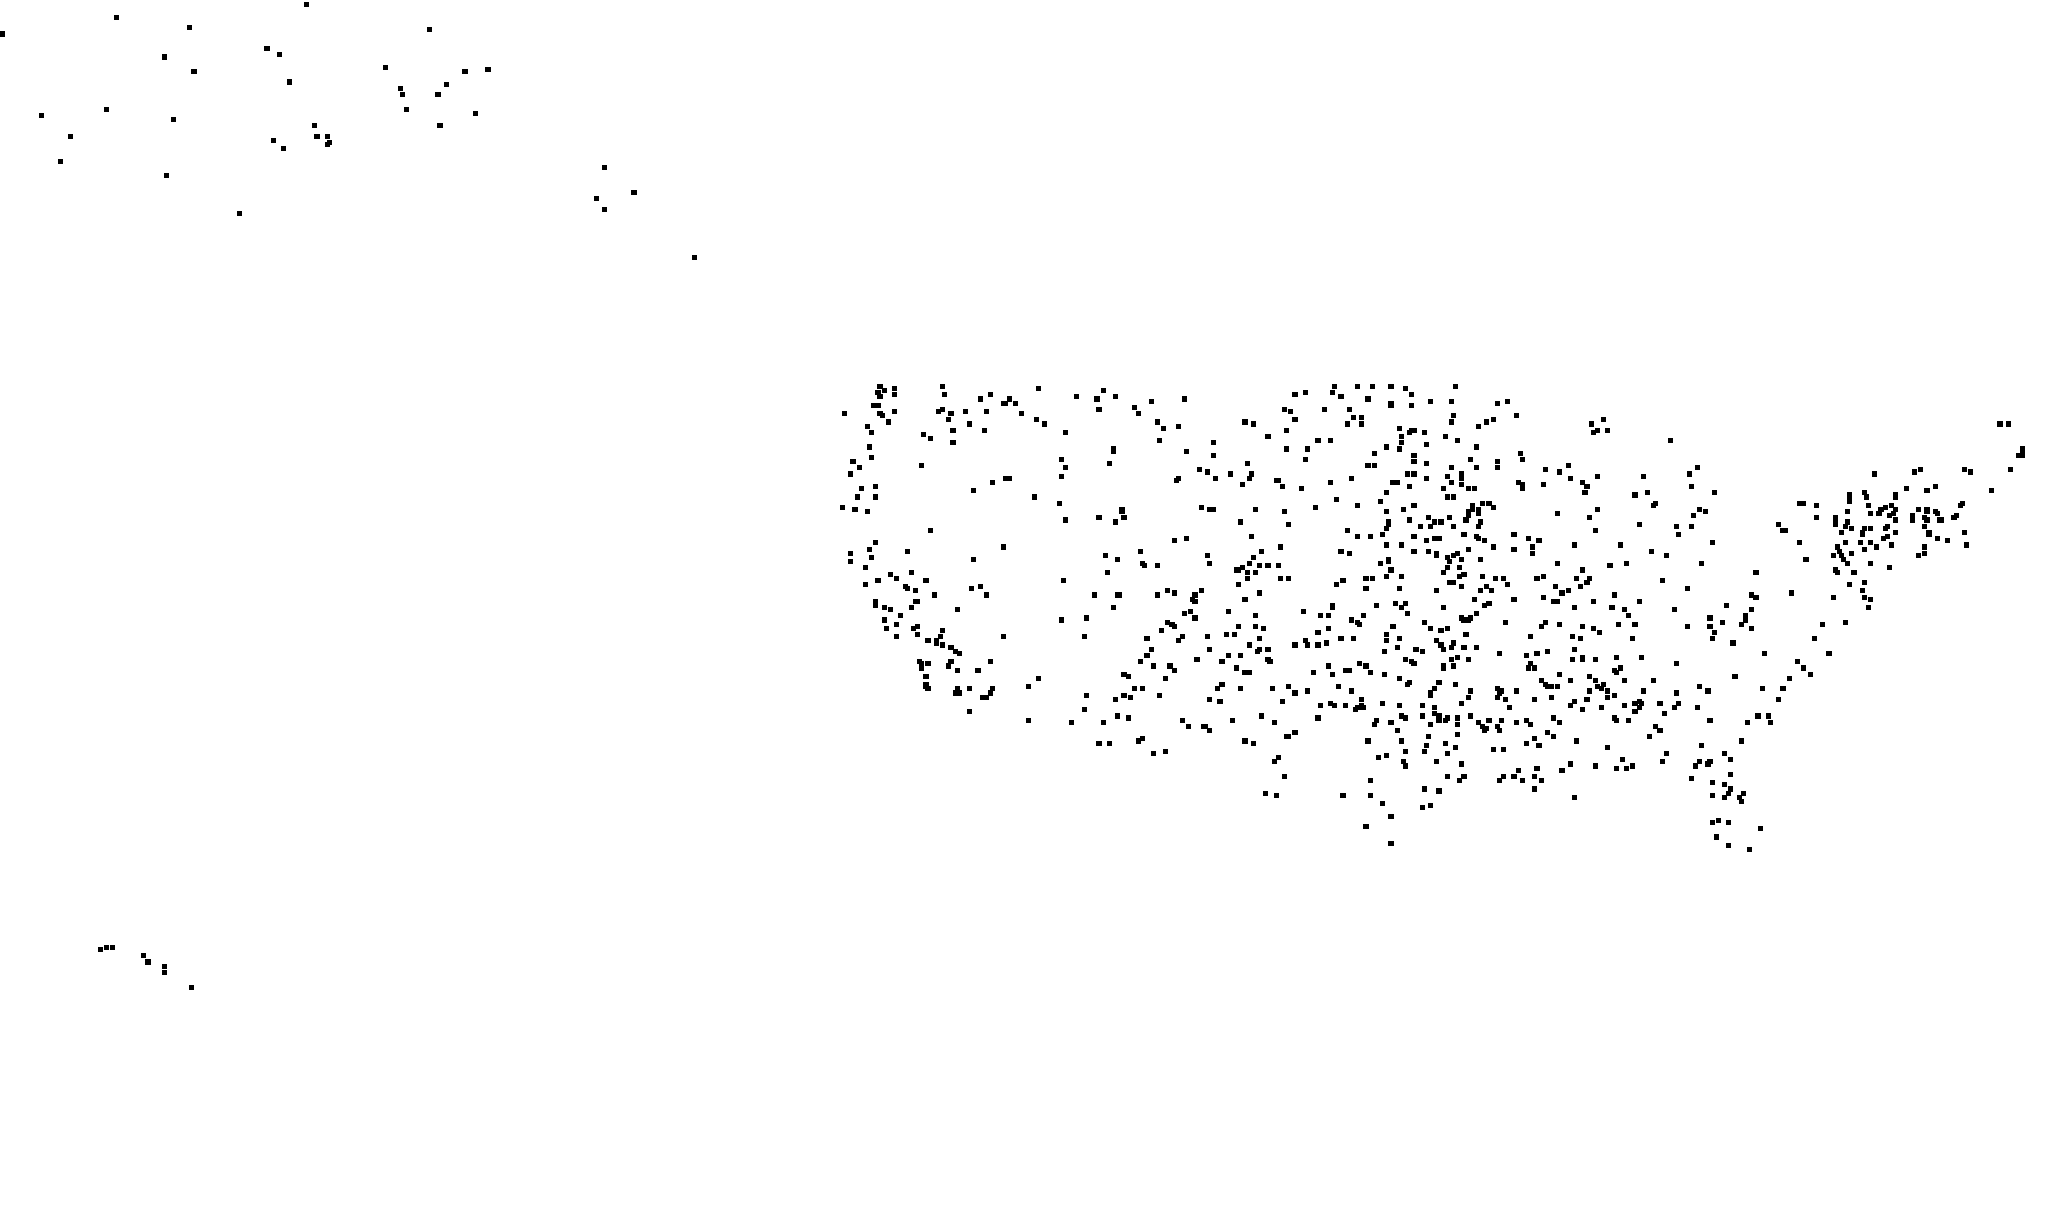
\includegraphics[width=\textwidth]{fig/uspp1k.pdf}
\caption{US points of populated places - 1k rectangles}
\label{fig:usdata1k}
\end{minipage}
\begin{minipage}{0.49\textwidth}
\centering
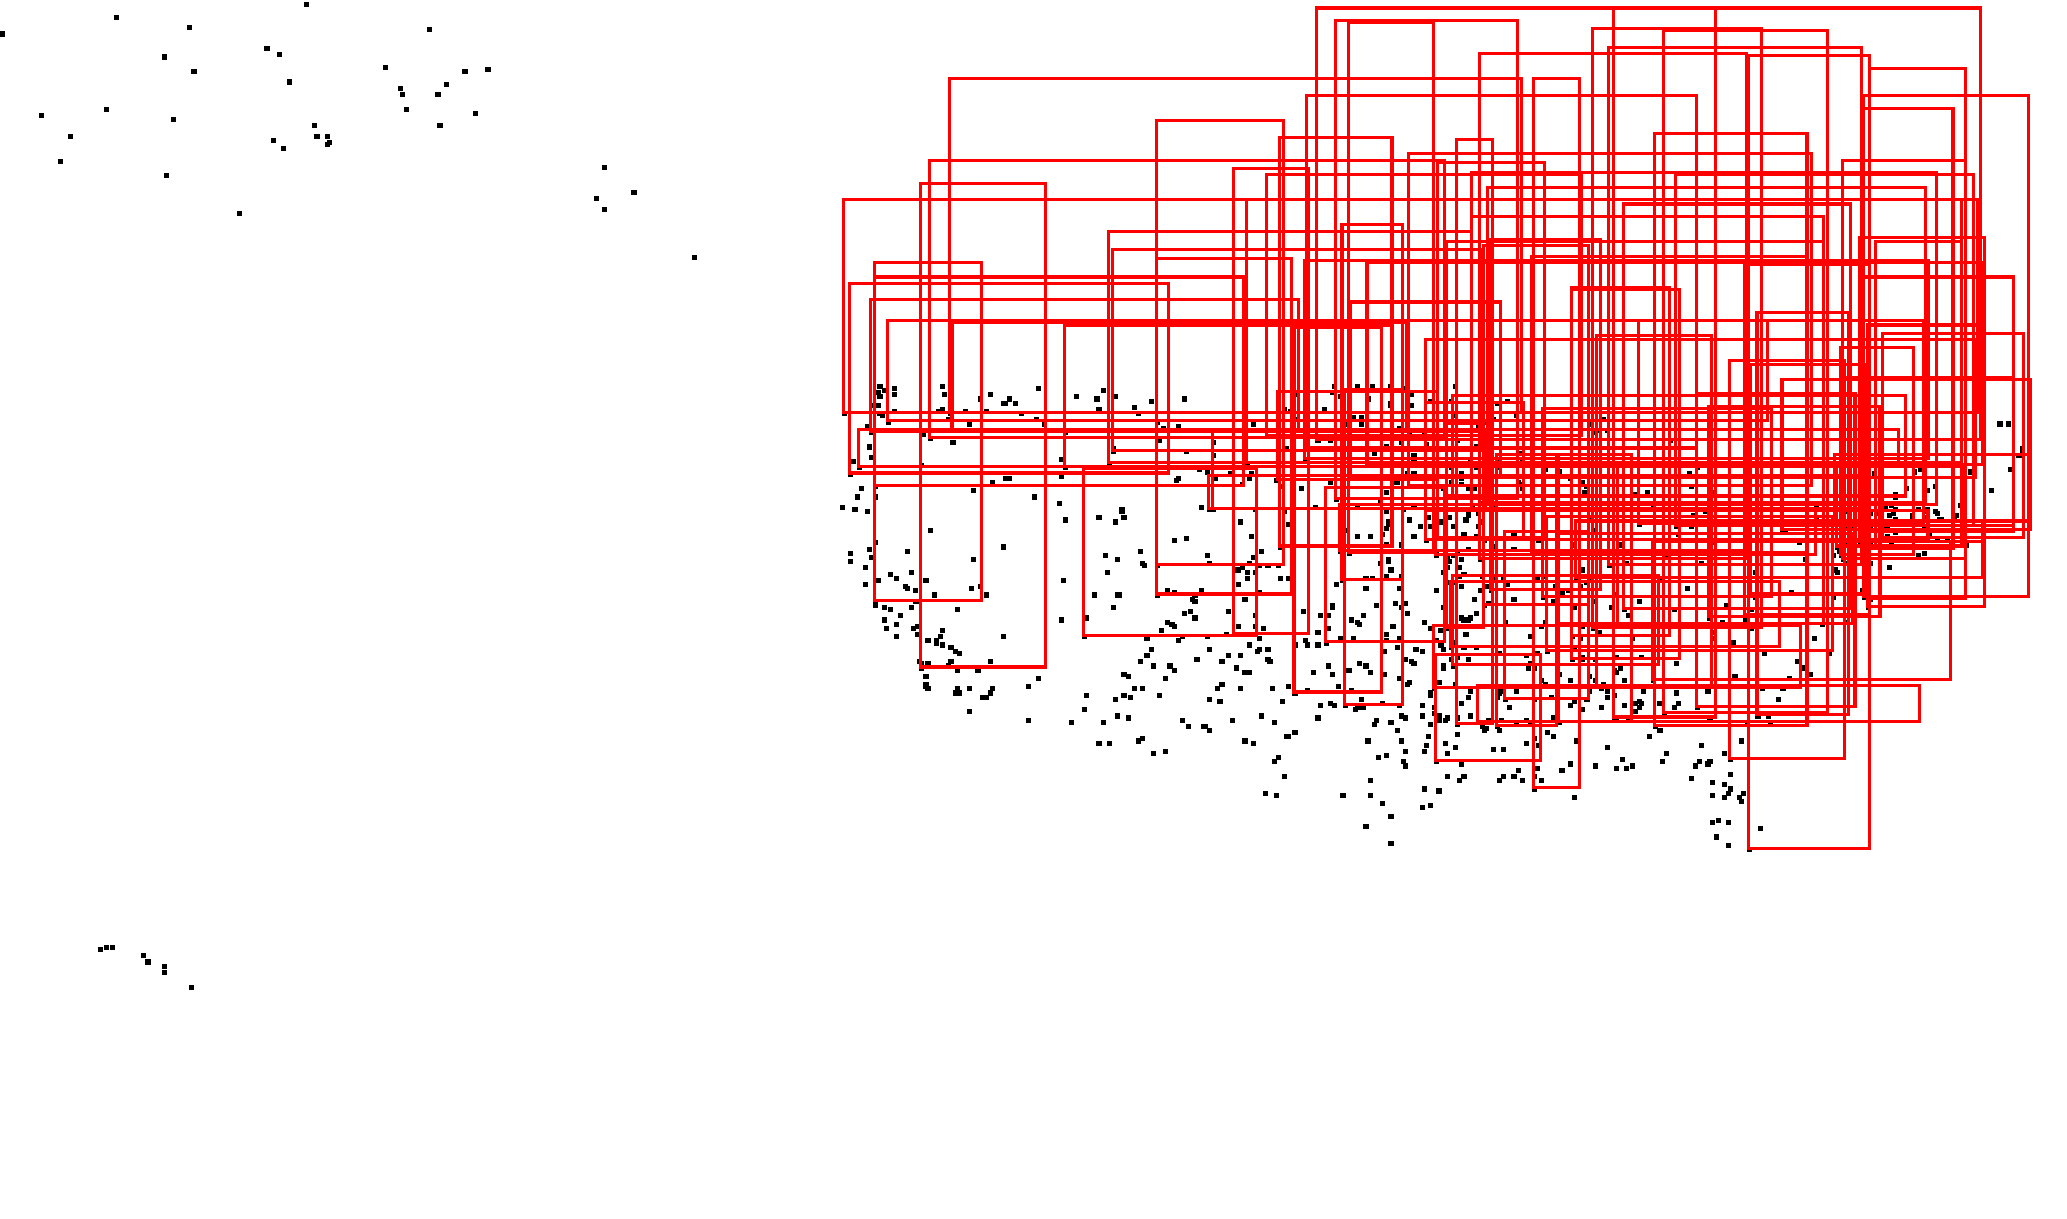
\includegraphics[width=\textwidth]{fig/uspp1kSearches.pdf}
\caption{US points of populated places - 1k rectangles - Search overlay}
\label{fig:usdataSearch}
\end{minipage}
\end{figure}


\paragraph{Proxy 1}
The first experiment tests insert and delete performance of the three algorithms. We sampled the last 10\% of all insert and every 10th of all delete operations and took the average result of the operations sampled. 

We expect the linear algorithm to outperform the others and the exhaustive algorithm to perform the worst. However, insert cost is mainly determined by frequency of node splits. In case the sampled insert operations contained few or no node splits, this result can be biased. In the original paper, for example, the last 10\% of insert operations were measured. In case the data set to be inserted being sorted, we could observe little to no variance for the insert operations sampled, and even encounter a surprise with the exhaustive algorithm. Given that the exhaustive algorithm will find an optimal split, further splits may not be necessary in the last 10\% of insert operations, hence it would perform equally well or even better than the linear algorithm. If the input data set is randomized, however, we expect to see the linear algorithm outperform the quadratic algorithm, which should outperform the exhaustive algorithm. For smaller page sizes, the quadratic algorithm may perform similarly well to the linear algorithm, since the overhead of reorganizing entry lists during a node split could outweigh the runtime difference of the actual list split algorithm.

\paragraph{Proxy 2}
The second hypothesis can be tested with the same experimental setup as the first.

We expect to see exactly that - at least some increased insert performance for more strict node-fill criteria, but some decreased delete performance, particularly for smaller page sizes. The result can be impacted by sample data bias, if, for example, the majority of sampled delete operations did not lead to split operations. 

\paragraph{Proxy 3}
The experimental setup for testing the third hypothesis involves running 100 search operations each of which returns between 4 and 6\% of the data. We measured CPU time required for each search operation,  divided by the number of search results, and averaged over the 100 operations. 

For experiments testing this hypothesis we expect to see similar results for the three different split algorithms. 

\paragraph{Proxy 4}
For testing this hypothesis, we measured the amount of memory used by trees containing the same data but built using different node-fill criteria. We did this for all three of the node split algorithms and different page sizes.

We expect to see less memory consumption for trees with more strict node-fill criteria. Besides we expect to see the exhaustive algorithm to require the least amount of space (as optimal splits are achieved), with quadratic and linear algorithm possibly being tied, or the quadratic algorithm outperforming the linear one, as the random entry reorganization of the linear split algorithm can lead to a less organized tree structure. 

\paragraph{Proxy 5}
We measured insert and delete performance for trees built with varying numbers of elements. 

We expect to see jumps in the graph where tree level changes but unchanged performance for different element numbers accommodated in trees of the same height.

\paragraph{Proxy 6}
We measured search cost (number of page accesses and CPU time) for 100 searches each returning between 3 and 6\% of all data for each of the data sets containing between 1000 and 5000 data records.

We expect the search cost per qualifying record to decrease with increase of the number of elements as search effort will amortize and tree traversal becomes less relevant.

\paragraph{Proxy 7}
To test the last hypothesis, we measured space consumption for trees containing varying numbers of elements, from 1000 elements up to 5000.

We expect space consumption to linearly increase with the number of elements.

\subsection{Experimental Results and Discussion}
This subsection presents the results of the experiments previously described. On the left hand side of each experimental result figure we see the results of the random data set, depicted on the right hand side are the results of the US points of popular places data set.

\begin{figure}[h]
\centering
\begin{minipage}{0.49\textwidth}
\centering
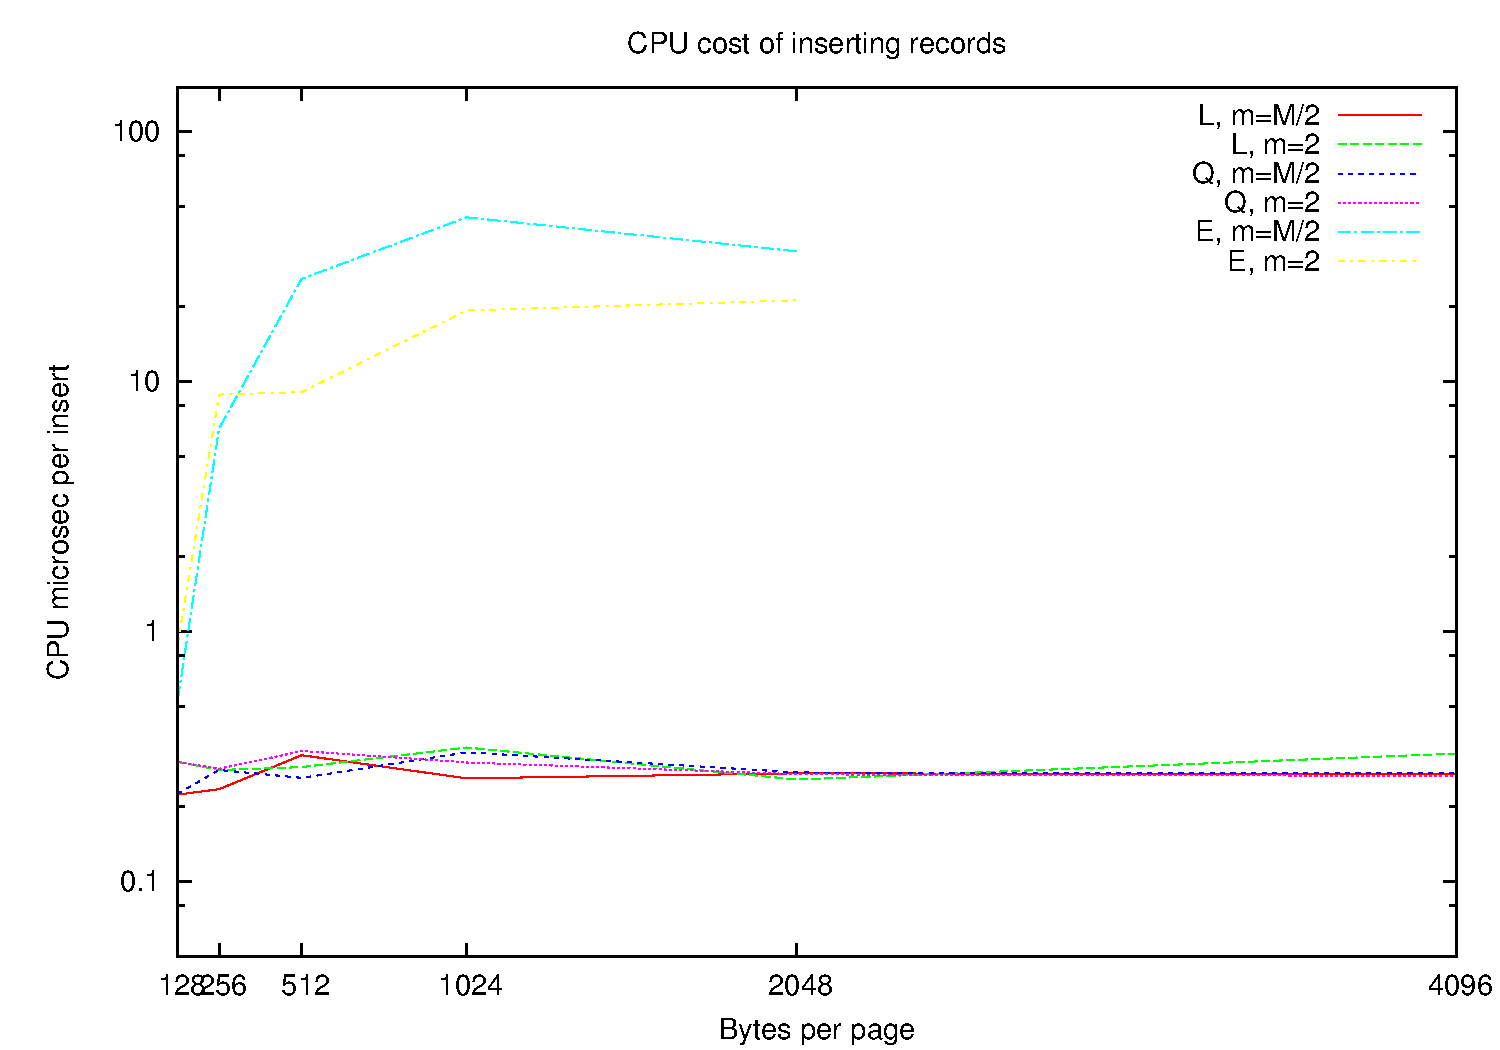
\includegraphics[width=\textwidth]{fig/random/figure-4-2.pdf}
\end{minipage}
\begin{minipage}{0.49\textwidth}
\centering
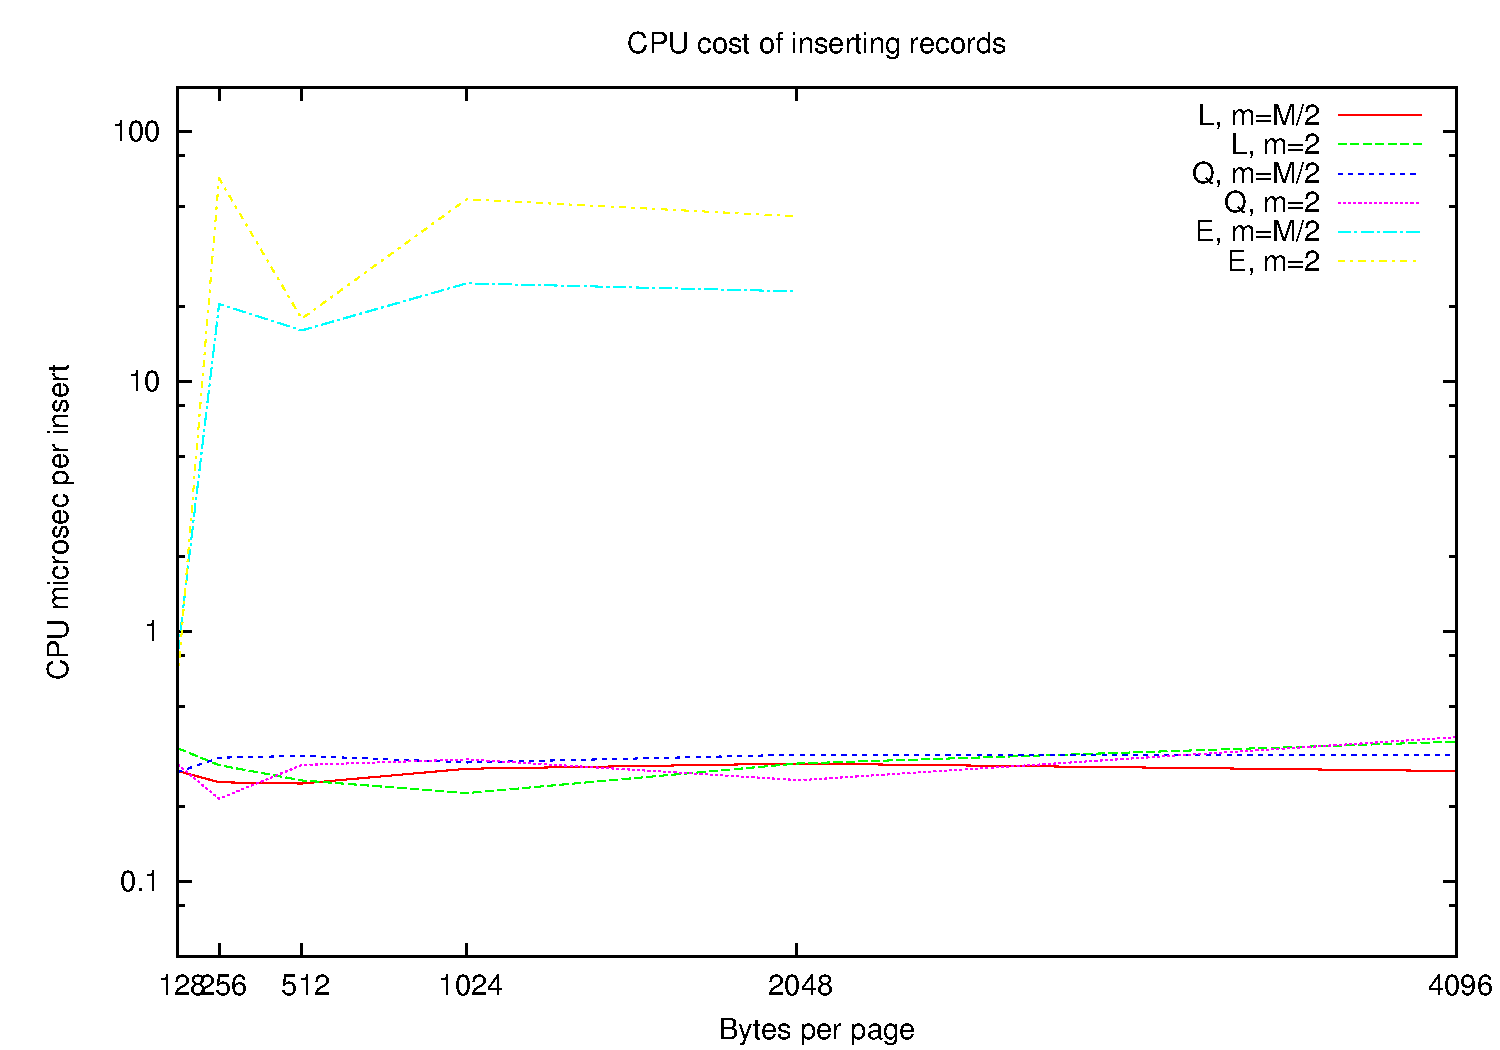
\includegraphics[width=\textwidth]{fig/usppp/figure-4-2.pdf}
\end{minipage}
\caption{CPU cost of inserting records}
\label{fig:4.2}
\end{figure}

\begin{figure}
\centering
\begin{minipage}{0.49\textwidth}
\centering
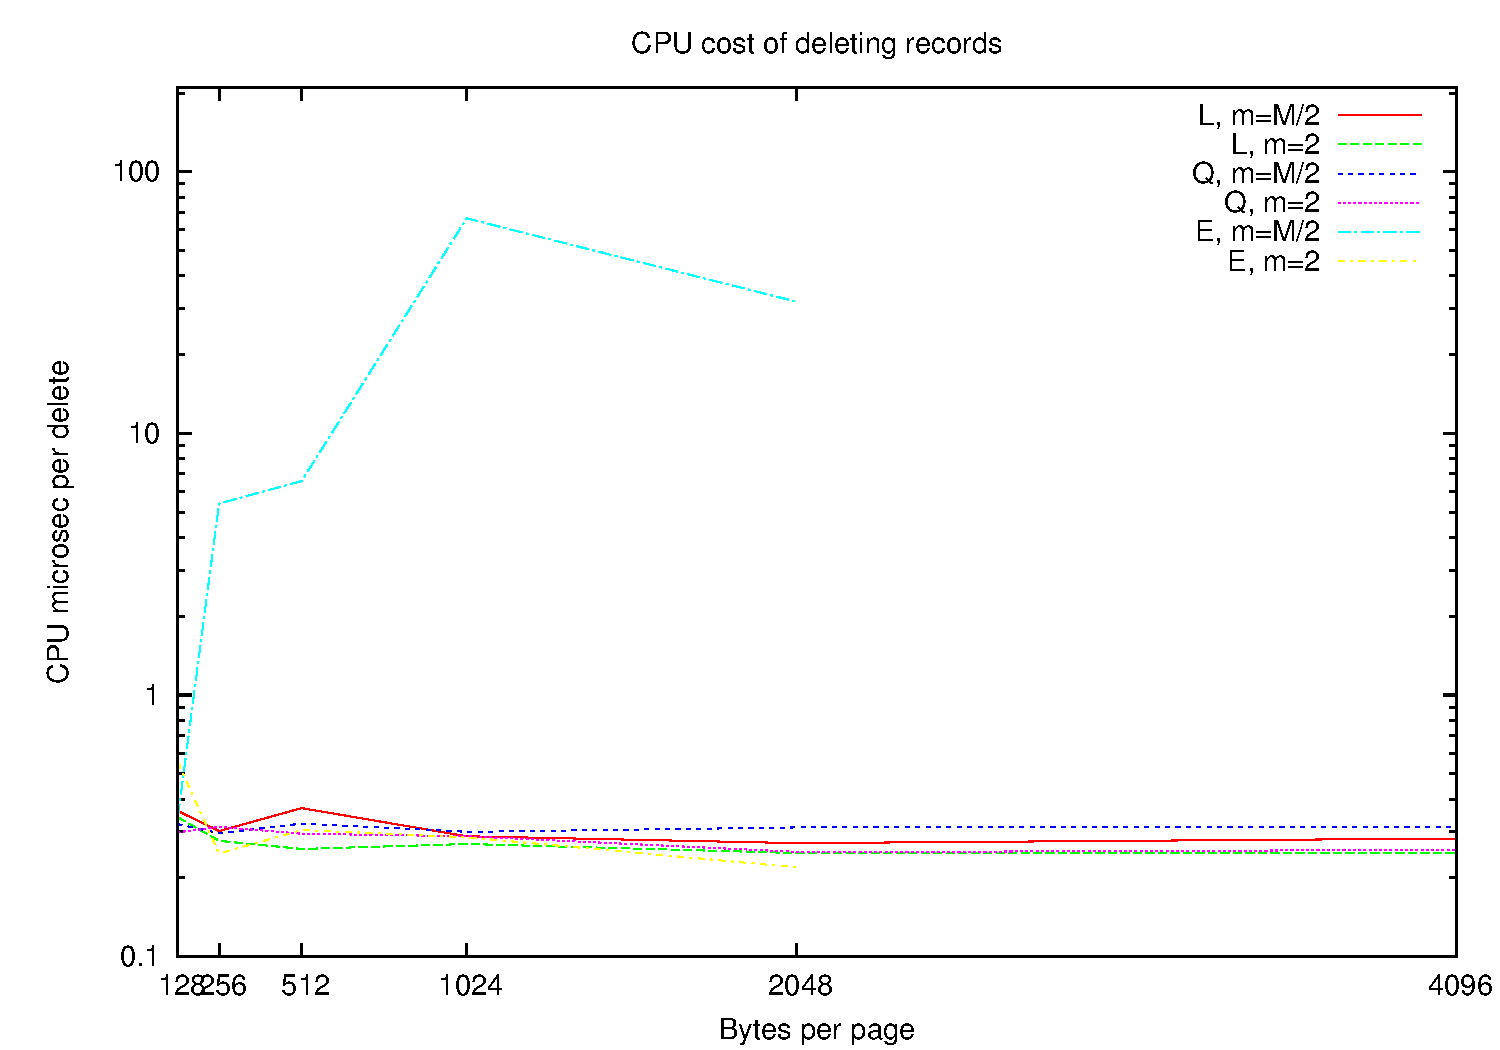
\includegraphics[width=\textwidth]{fig/random/figure-4-3.pdf}
\end{minipage}
\begin{minipage}{0.49\textwidth}
\centering
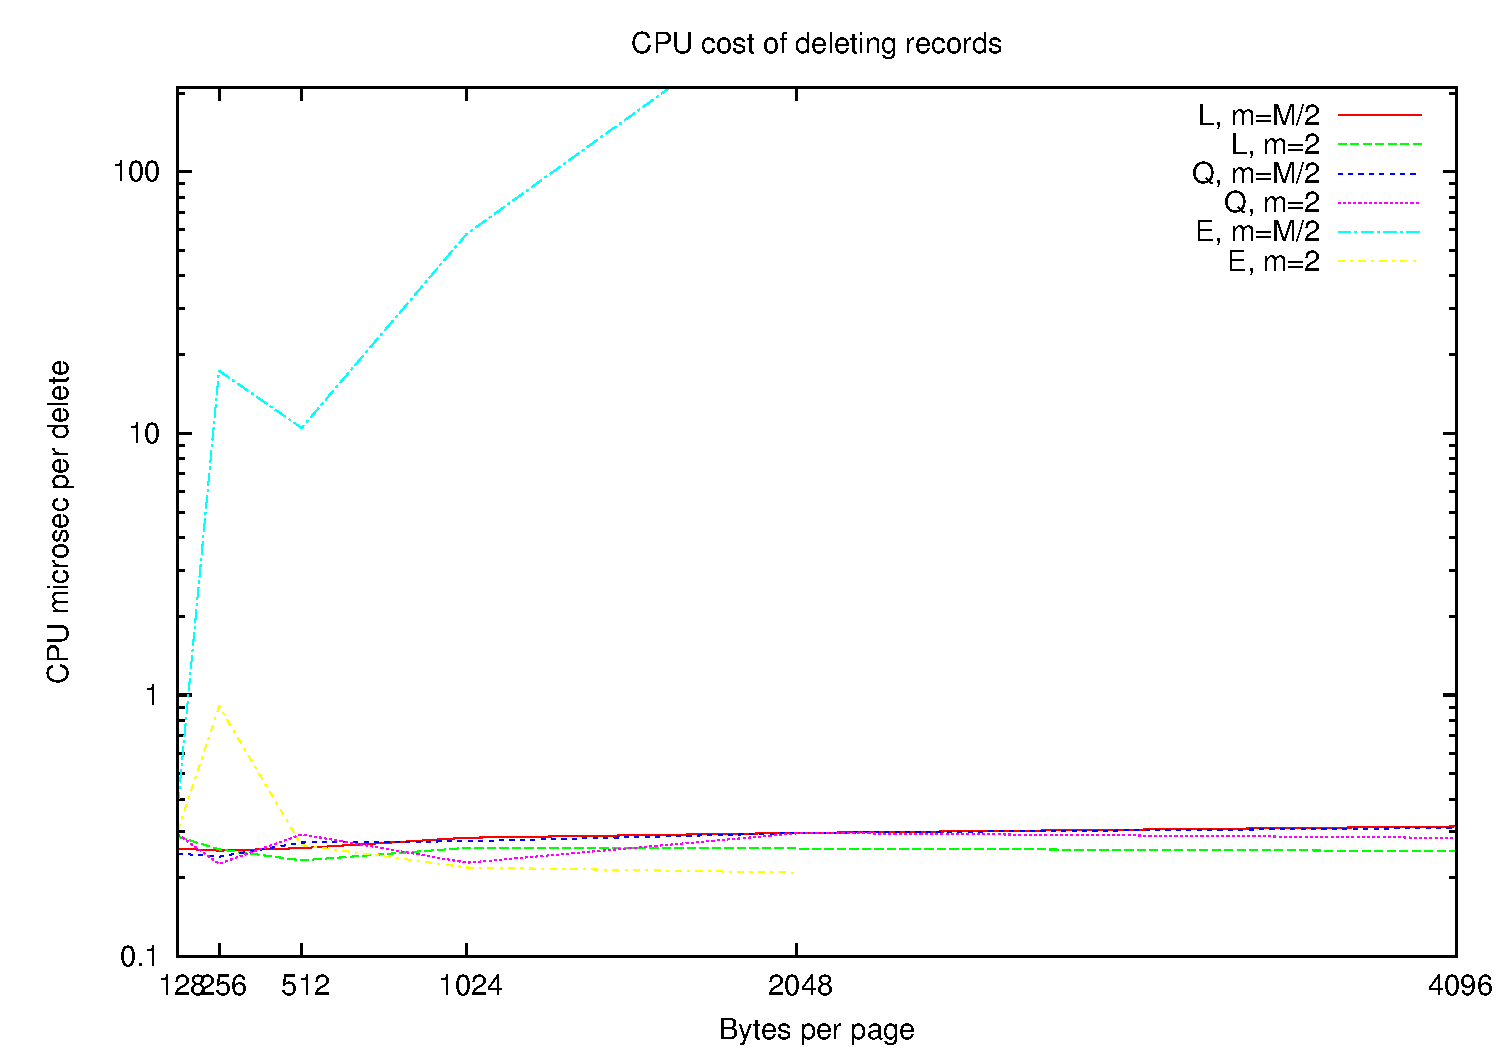
\includegraphics[width=\textwidth]{fig/usppp/figure-4-3.pdf}
\end{minipage}
\caption{CPU cost of deleting records}
\label{fig:4.3}
\end{figure}

Figures~\ref{fig:4.2} and \ref{fig:4.3} show insert and delete performance for the three different algorithms. We can clearly see that insert performance of the exhaustive algorithm is two orders of magnitudes worse than the performance of the other two algorithms. Delete performance for the exhaustive algorithm with less strict node-fill criterion is for most page sizes comparable to the other setups, since not many node splits occurred. Quadratic and linear algorithms  have comparable performance. The same holds true for different node-fill criteria. We only see a minor difference in performance for the more strict criteria for inserts and less strict criteria for deletes, especially for smaller page sizes. We assume that this is due to operational overhead in STL containers, such that the actual split algorithm run time is not significant anymore. The occasional peak can be explained through variable numbers of splits in the sampled operations. 

\begin{figure}
\centering
\begin{minipage}{0.49\textwidth}
\centering
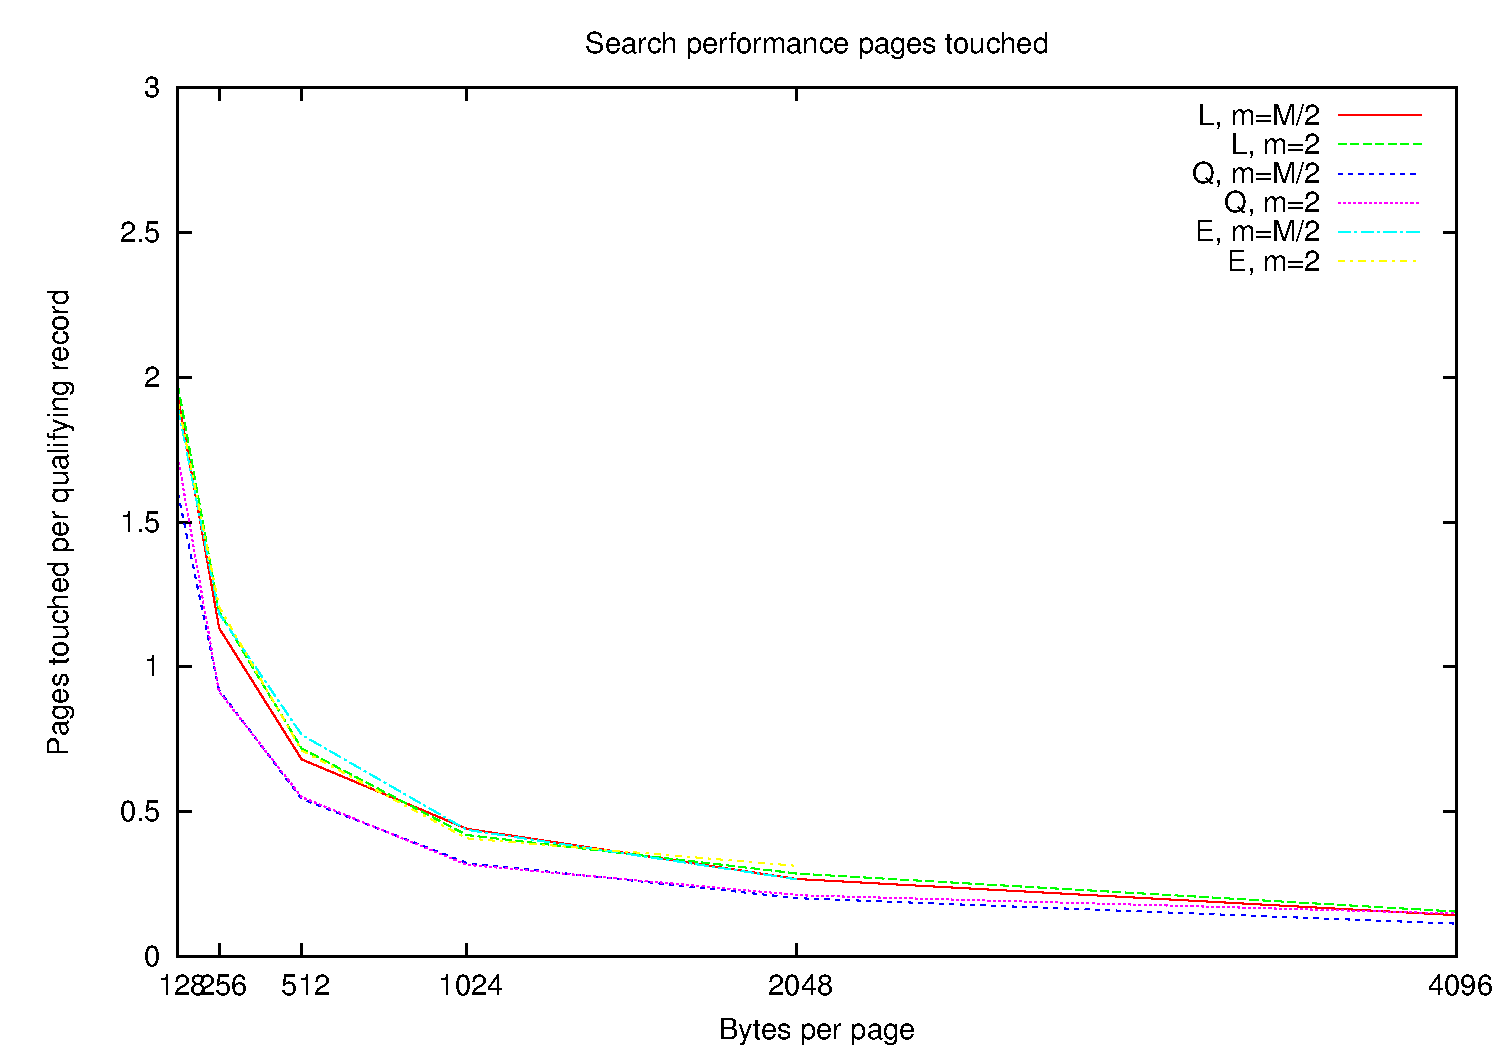
\includegraphics[width=\textwidth]{fig/random/figure-4-4.pdf}
\end{minipage}
\begin{minipage}{0.49\textwidth}
\centering
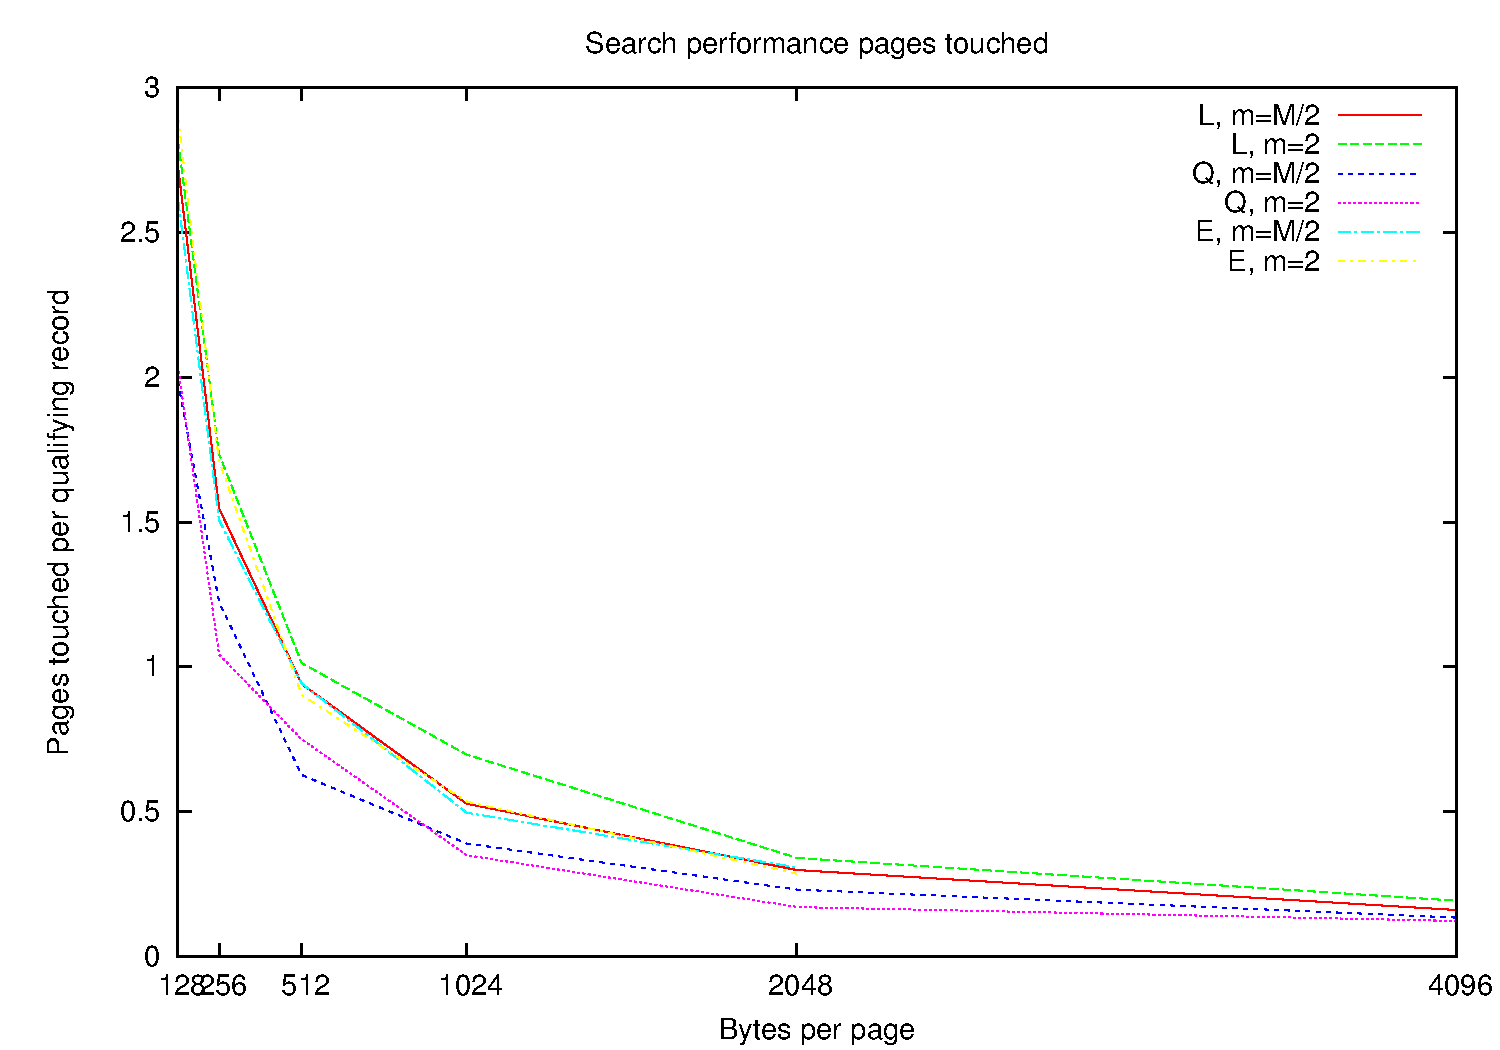
\includegraphics[width=\textwidth]{fig/usppp/figure-4-4.pdf}
\end{minipage}
\caption{Search performance - Pages touched}
\label{fig:4.4}
\end{figure}

\begin{figure}
\centering
\begin{minipage}{0.49\textwidth}
\centering
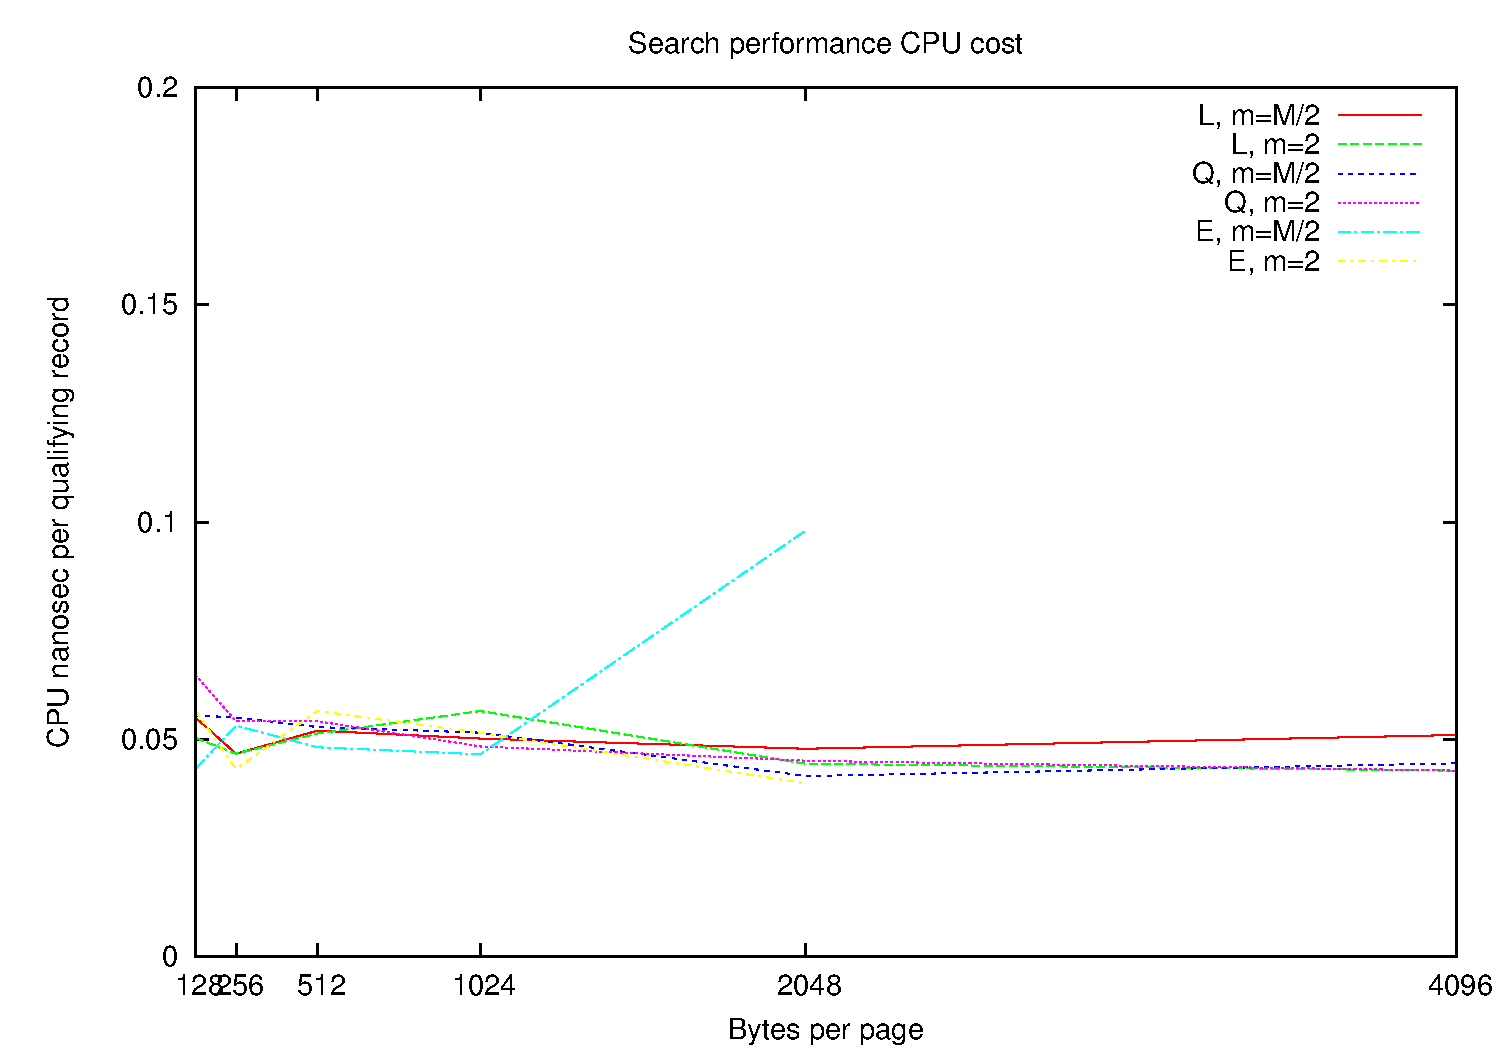
\includegraphics[width=\textwidth]{fig/random/figure-4-5.pdf}
\end{minipage}
\begin{minipage}{0.49\textwidth}
\centering
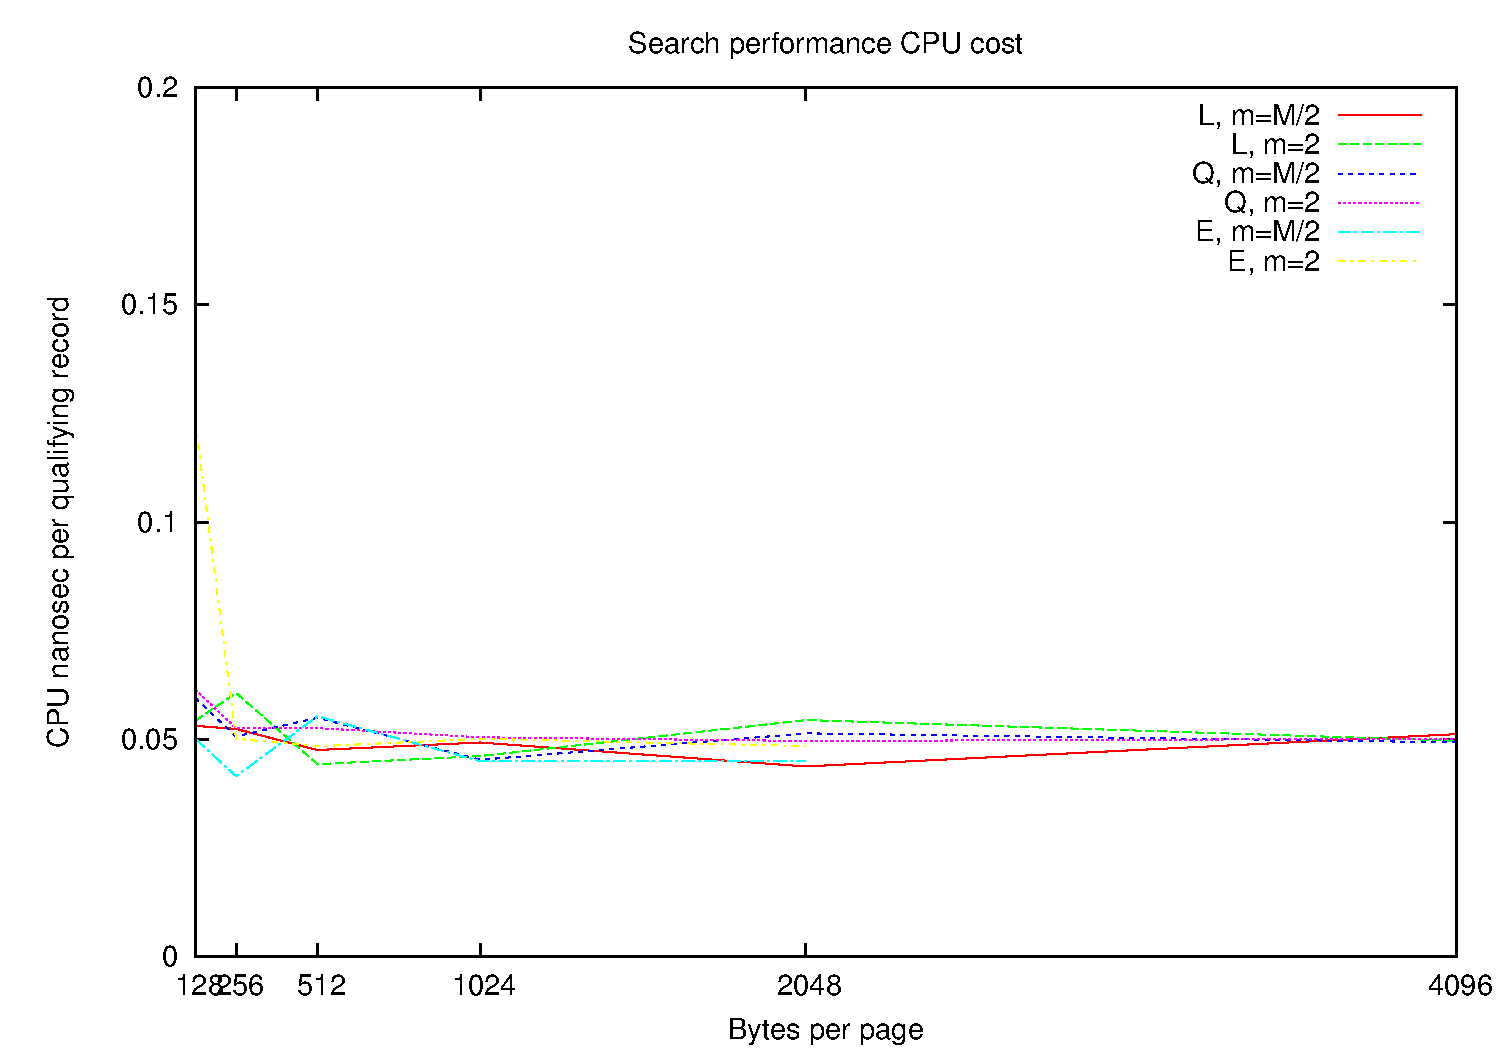
\includegraphics[width=\textwidth]{fig/usppp/figure-4-5.pdf}
\end{minipage}
\caption{Search performance - CPU cost}
\label{fig:4.5}
\end{figure}

Search performance is shown in figures~\ref{fig:4.4} and \ref{fig:4.5}. The experiments indeed confirm the hypothesis that search performance is mostly insensitive to the choice of split algorithm. As expected, the exhaustive algorithm insignificantly outperforms the linear algorithm, due to more optimal node splits.

\begin{figure}
\centering
\begin{minipage}{0.49\textwidth}
\centering
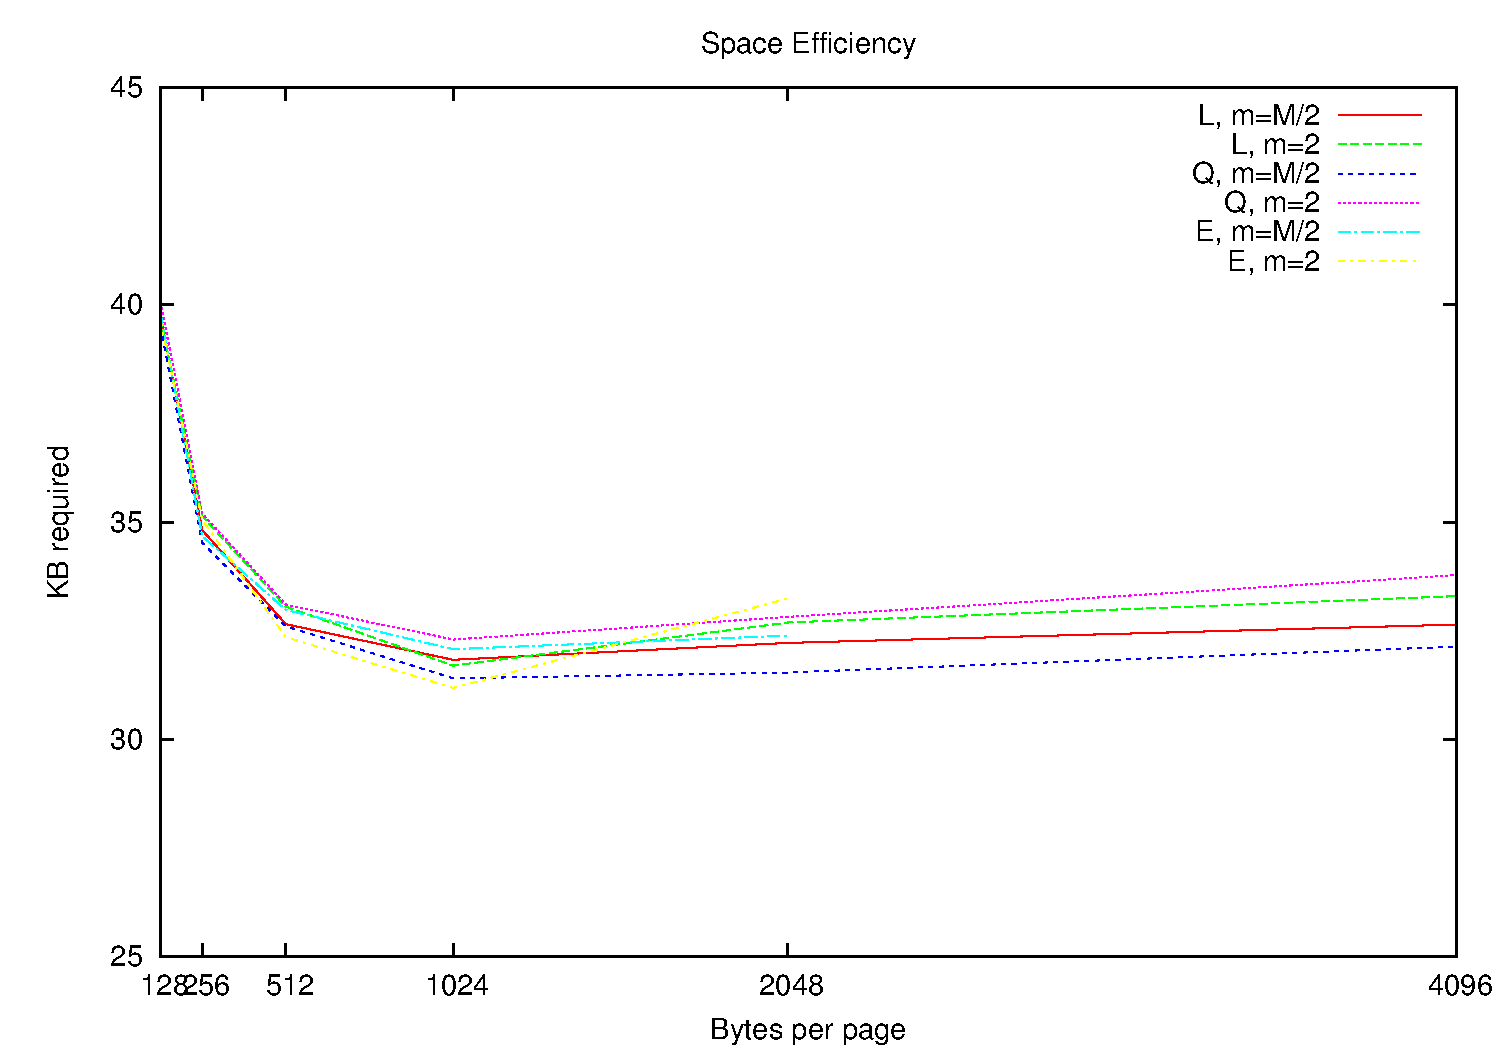
\includegraphics[width=\textwidth]{fig/random/figure-4-6.pdf}
\end{minipage}
\begin{minipage}{0.49\textwidth}
\centering
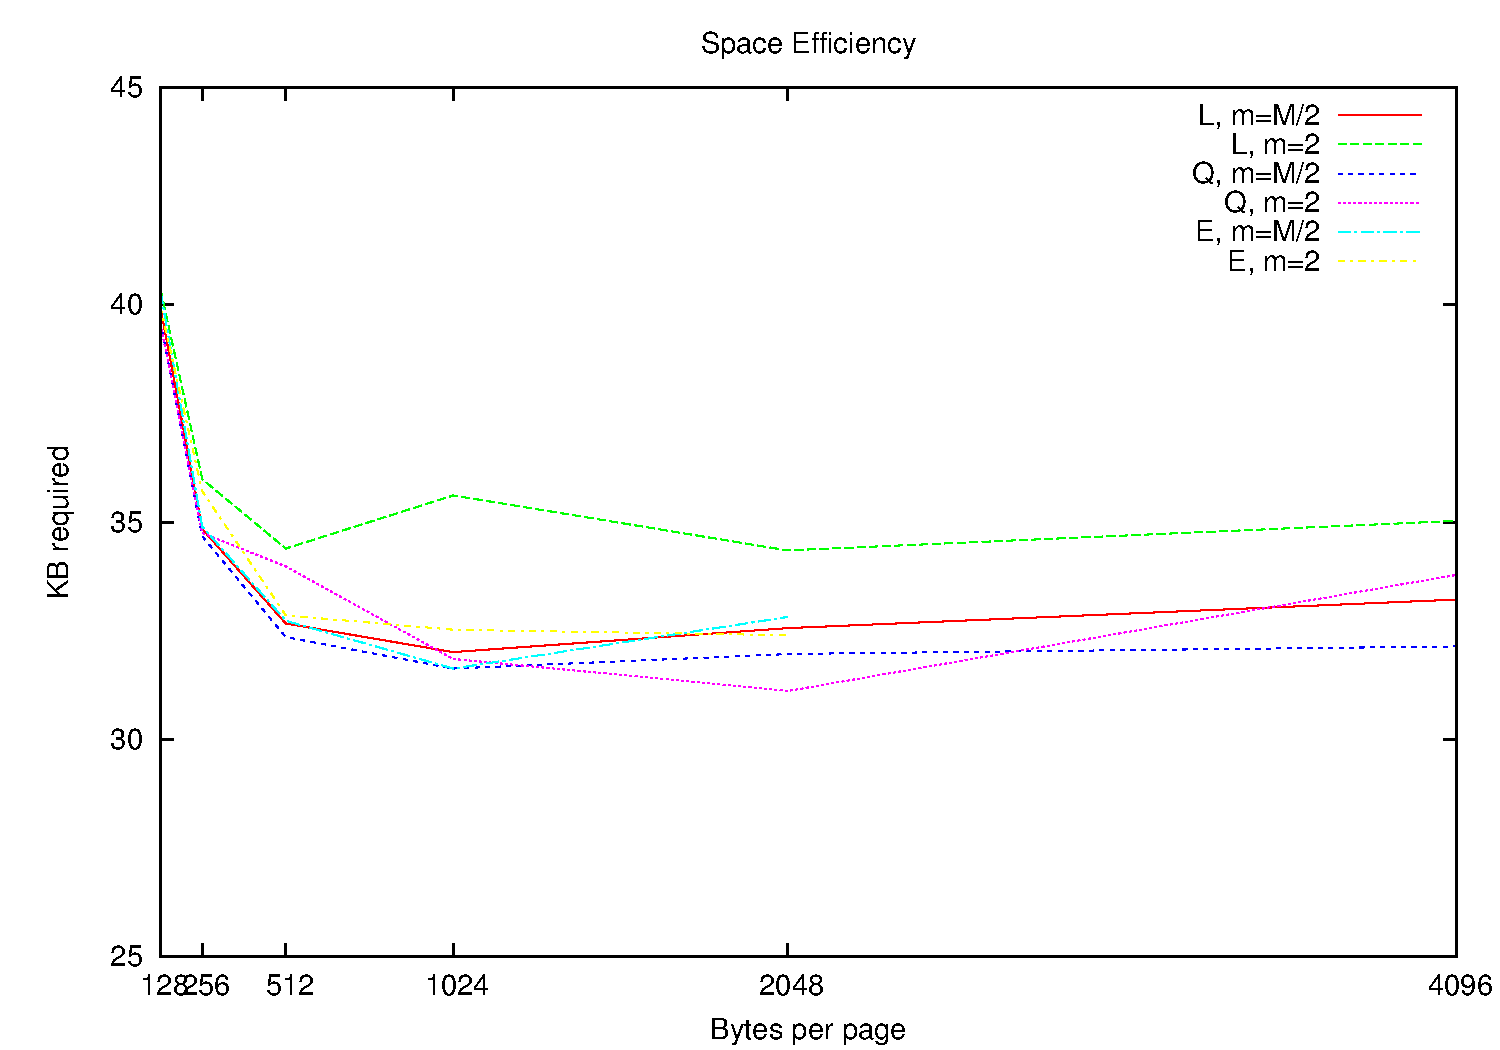
\includegraphics[width=\textwidth]{fig/usppp/figure-4-6.pdf}
\end{minipage}
\caption{Space efficiency}
\label{fig:4.6}
\end{figure}

Experimental results for space consumption are shown in figure~\ref{fig:4.6}. For plots of the same split algorithm it seems generally true that more strict node-fill criteria lead to less space consumption. The largest difference is less than 15\%, though. The fact that these results differ from the original paper could be explained by implementation details since out implemented version already uses less space than the original R-Tree.

\begin{figure}
\centering
\begin{minipage}{0.49\textwidth}
\centering
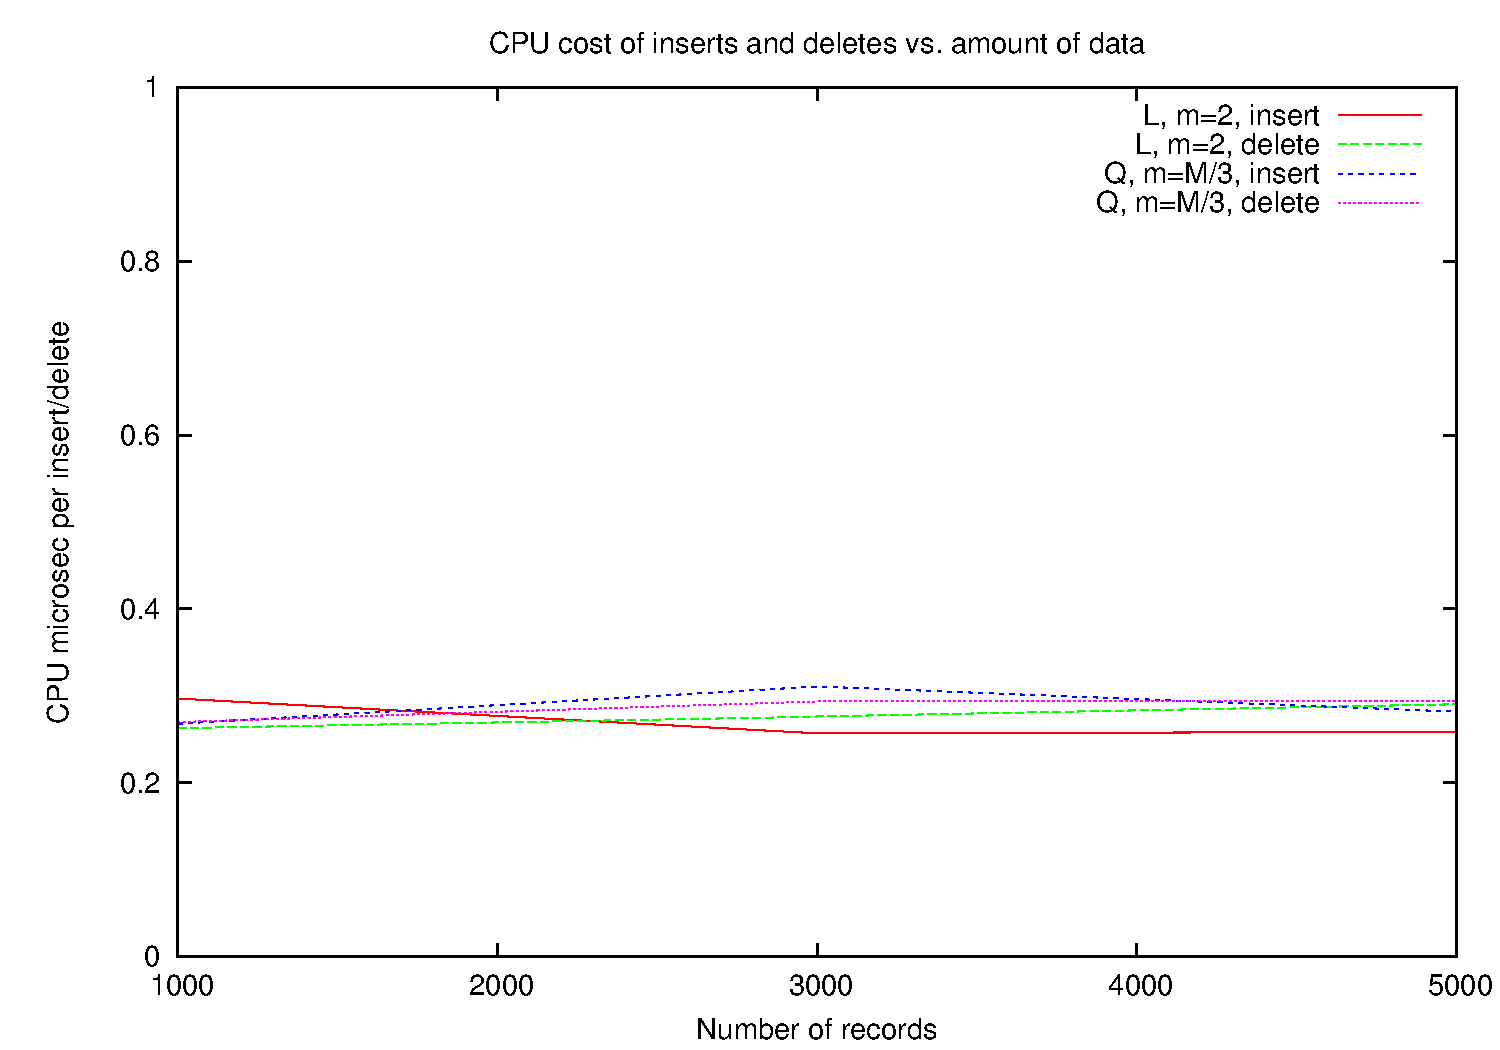
\includegraphics[width=\textwidth]{fig/random/figure-4-7.pdf}
\end{minipage}
\begin{minipage}{0.49\textwidth}
\centering
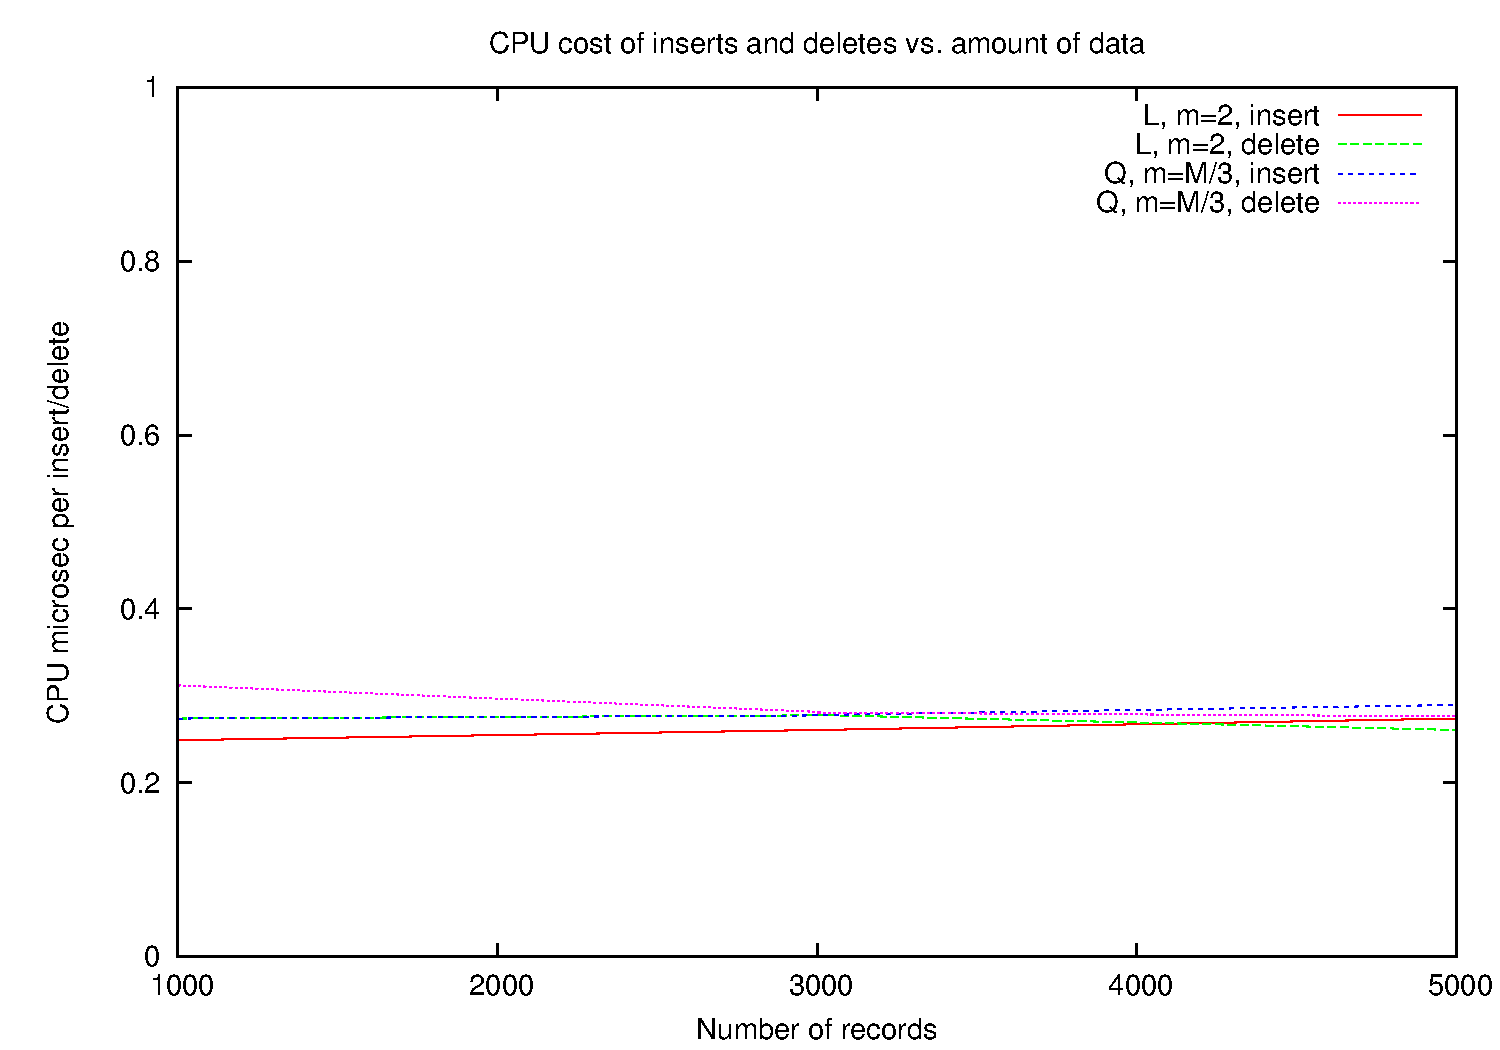
\includegraphics[width=\textwidth]{fig/usppp/figure-4-7.pdf}
\end{minipage}
\caption{CPU cost of insert and deletes vs amount of data}
\label{fig:4.7}
\end{figure}

In figure~\ref{fig:4.7} we see the CPU cost for insert and delete operations plotted against the amount of data in the tree. The graph shows us that the cost stays constant across changed number of tree elements, which contradicts our hypothesis. It however supports our claims from figures~\ref{fig:4.2} and ~\ref{fig:4.3} that, given modern processor speeds, the overhead created by maintaining STL containers could make the splits insignificant. Given that we received similar plots with different data randomization, we exclude data bias as a reason.

\begin{figure}
\centering
\begin{minipage}{0.49\textwidth}
\centering
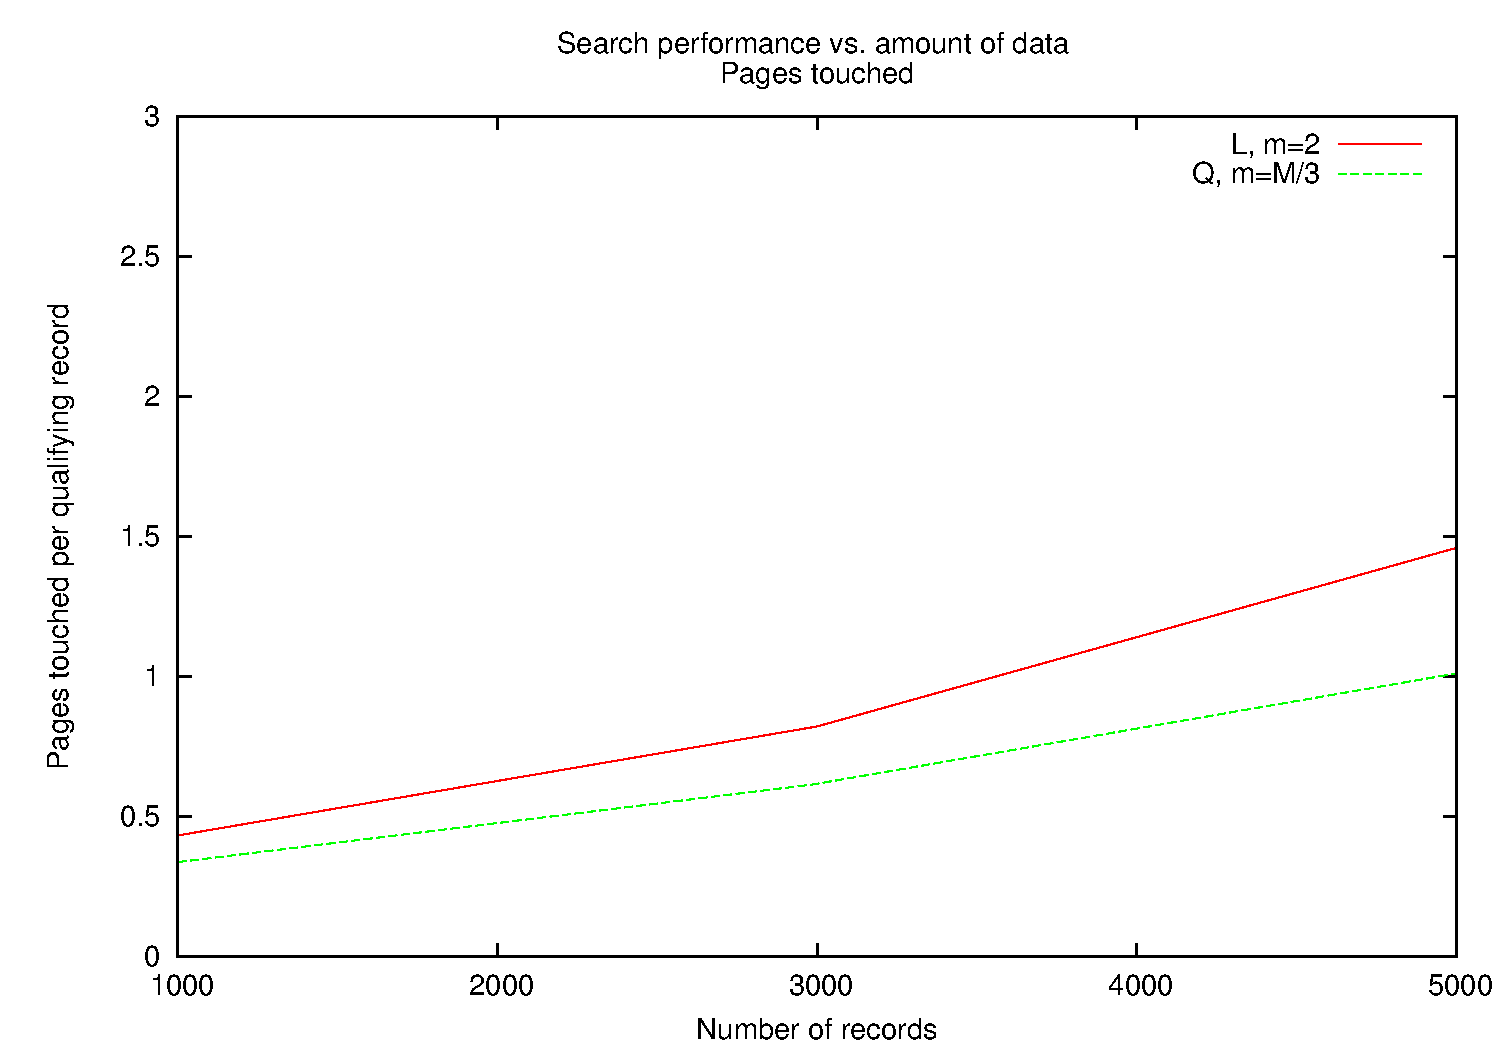
\includegraphics[width=\textwidth]{fig/random/figure-4-8.pdf}
\end{minipage}
\begin{minipage}{0.49\textwidth}
\centering
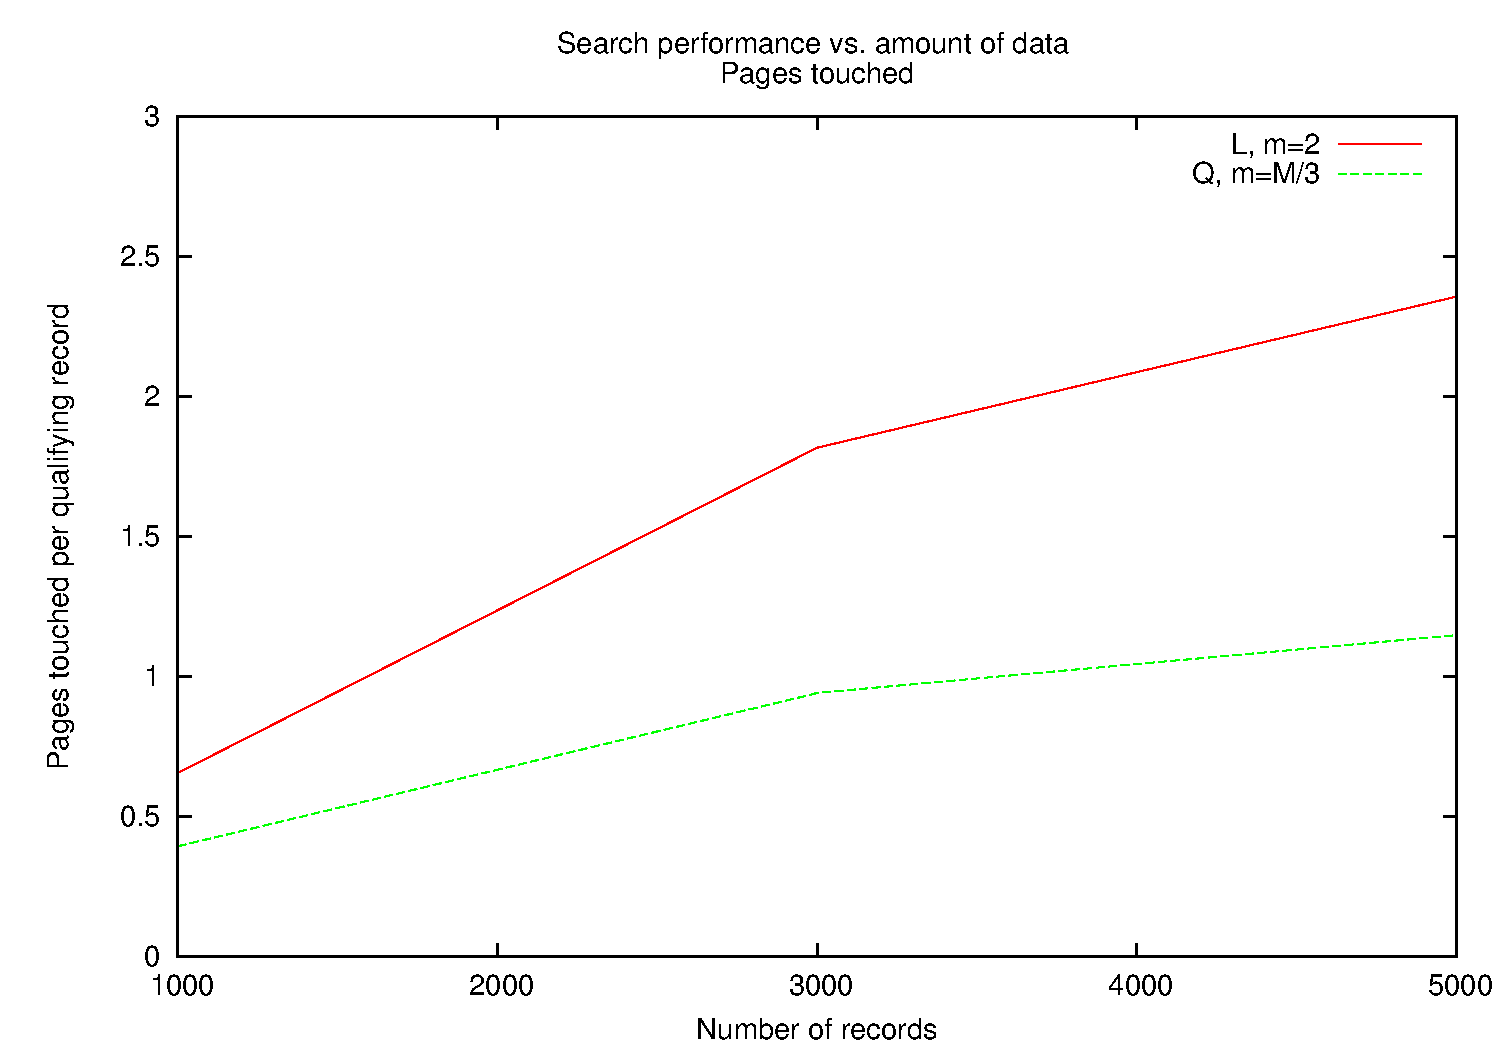
\includegraphics[width=\textwidth]{fig/usppp/figure-4-8.pdf}
\end{minipage}
\caption{Search performance vs amount of data - Pages touched}
\label{fig:4.8}
\end{figure}


\begin{figure}
\centering
\begin{minipage}{0.49\textwidth}
\centering
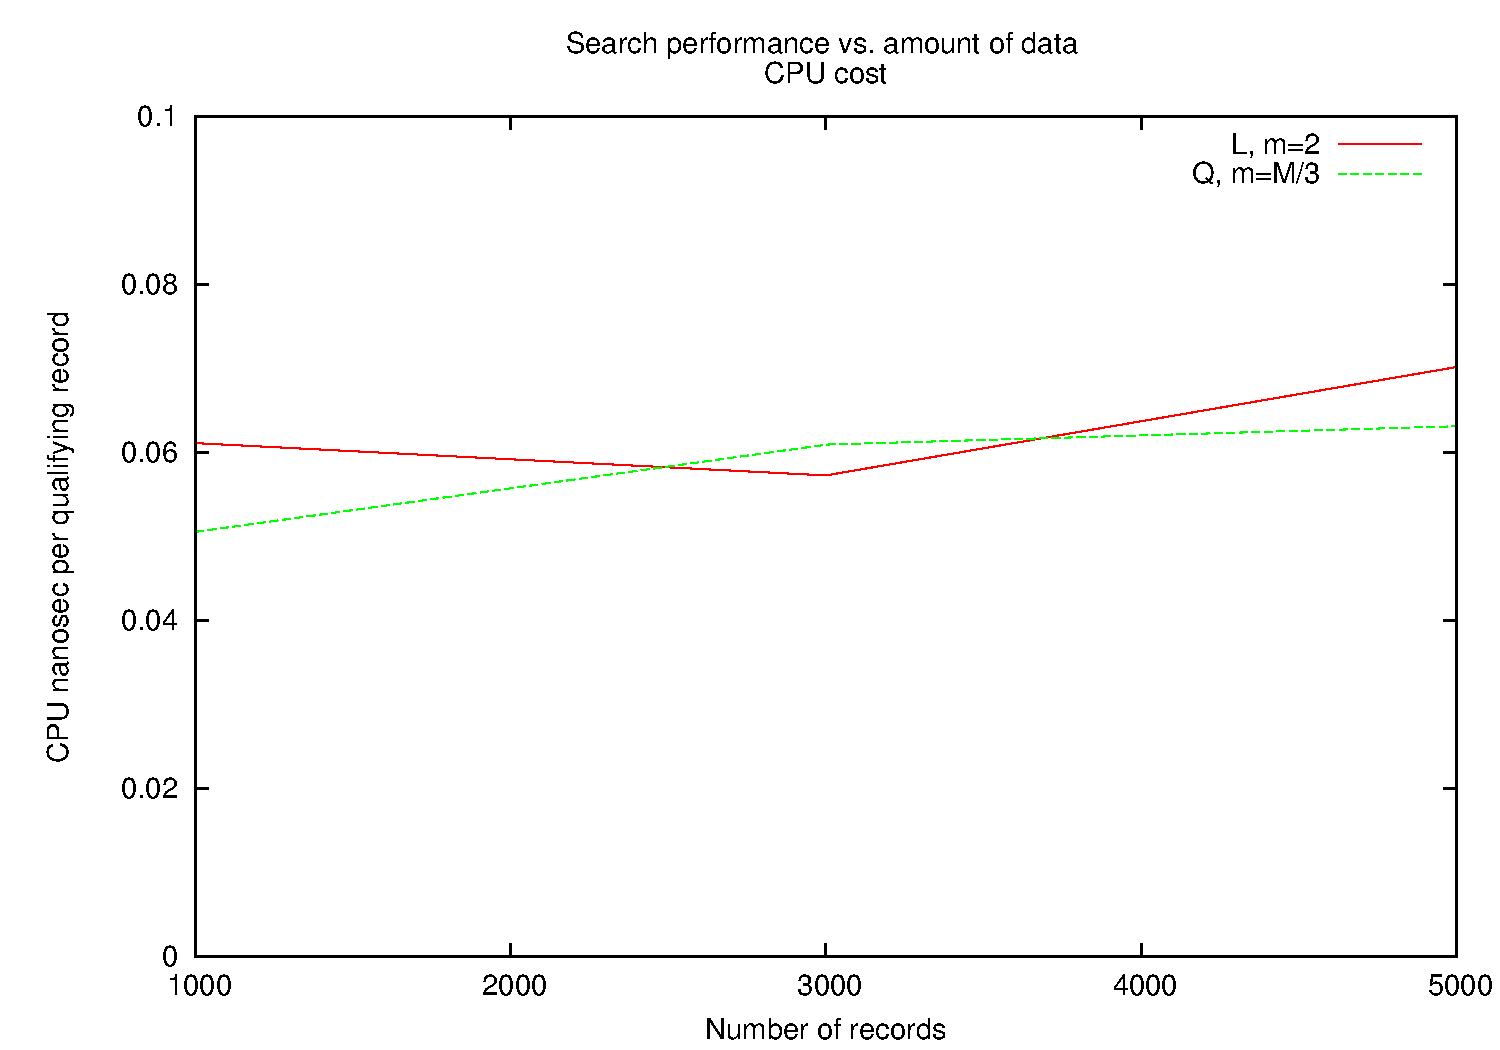
\includegraphics[width=\textwidth]{fig/random/figure-4-9.pdf}
\end{minipage}
\begin{minipage}{0.49\textwidth}
\centering
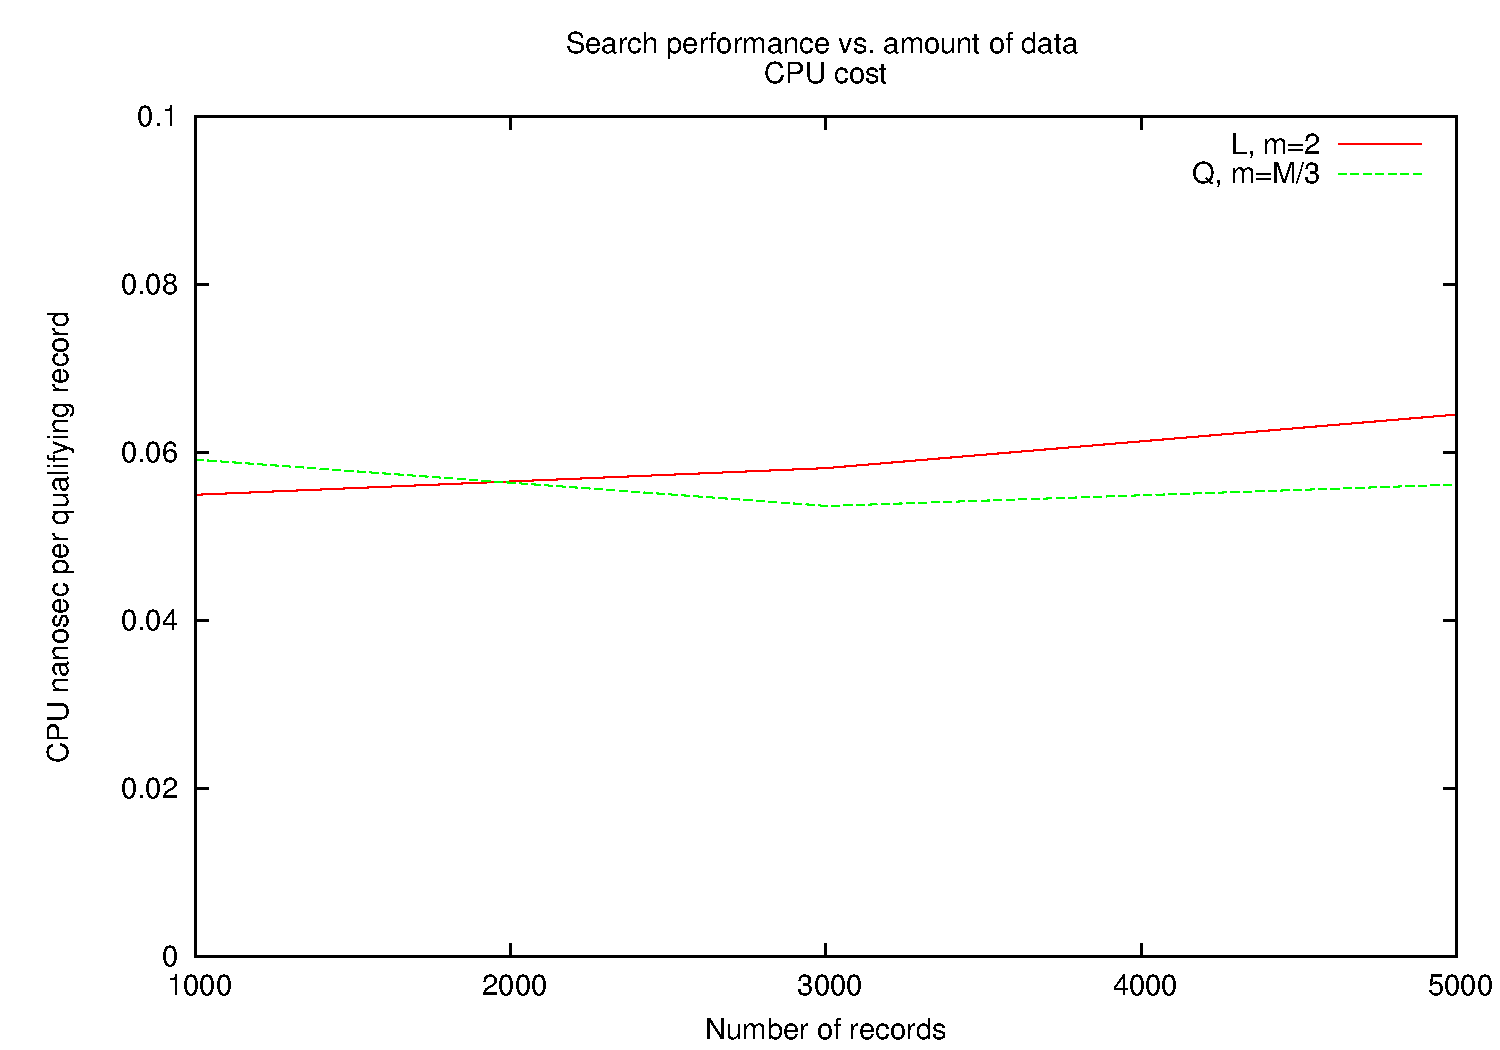
\includegraphics[width=\textwidth]{fig/usppp/figure-4-9.pdf}
\end{minipage}
\caption{Search performance vs amount of data - CPU cost}
\label{fig:4.9}
\end{figure}

Figures~\ref{fig:4.8} and \ref{fig:4.9} show search performance over change of numbers of records. We can see that the CPU cost shows some peaked variation but generally spoken remains fairly constant, a contradiction to what we see in the paper. Given that all searches return a fixed percentage of all data, it makes sense that possibly more leaf nodes have to be traversed to fulfill a search request. This assumption is supported by the graph showing the number of pages touched for different record numbers. More data stored in nodes of the same page size leads to more page traversals to retrieve fixed percentage search results. It also makes sense that the number of pages touched is higher for the sparse node-fill criterion of the linear algorithm, since this leads to a potentially larger number of leaf pages to visit in order to retrieve the final search result.

It is possible that the original paper reused the same search set for each of the trees, which is unclear from the original description. In case the percentage of data returned is not constant across all configurations, but instead the absolute number of search results is, the outcome in the original paper is entirely possible: more refined split intervals in the higher level lead to more direct paths to the leaf nodes, and in turn fewer higher-level nodes to traverse.  

\begin{figure}
\centering
\begin{minipage}{0.49\textwidth}
\centering
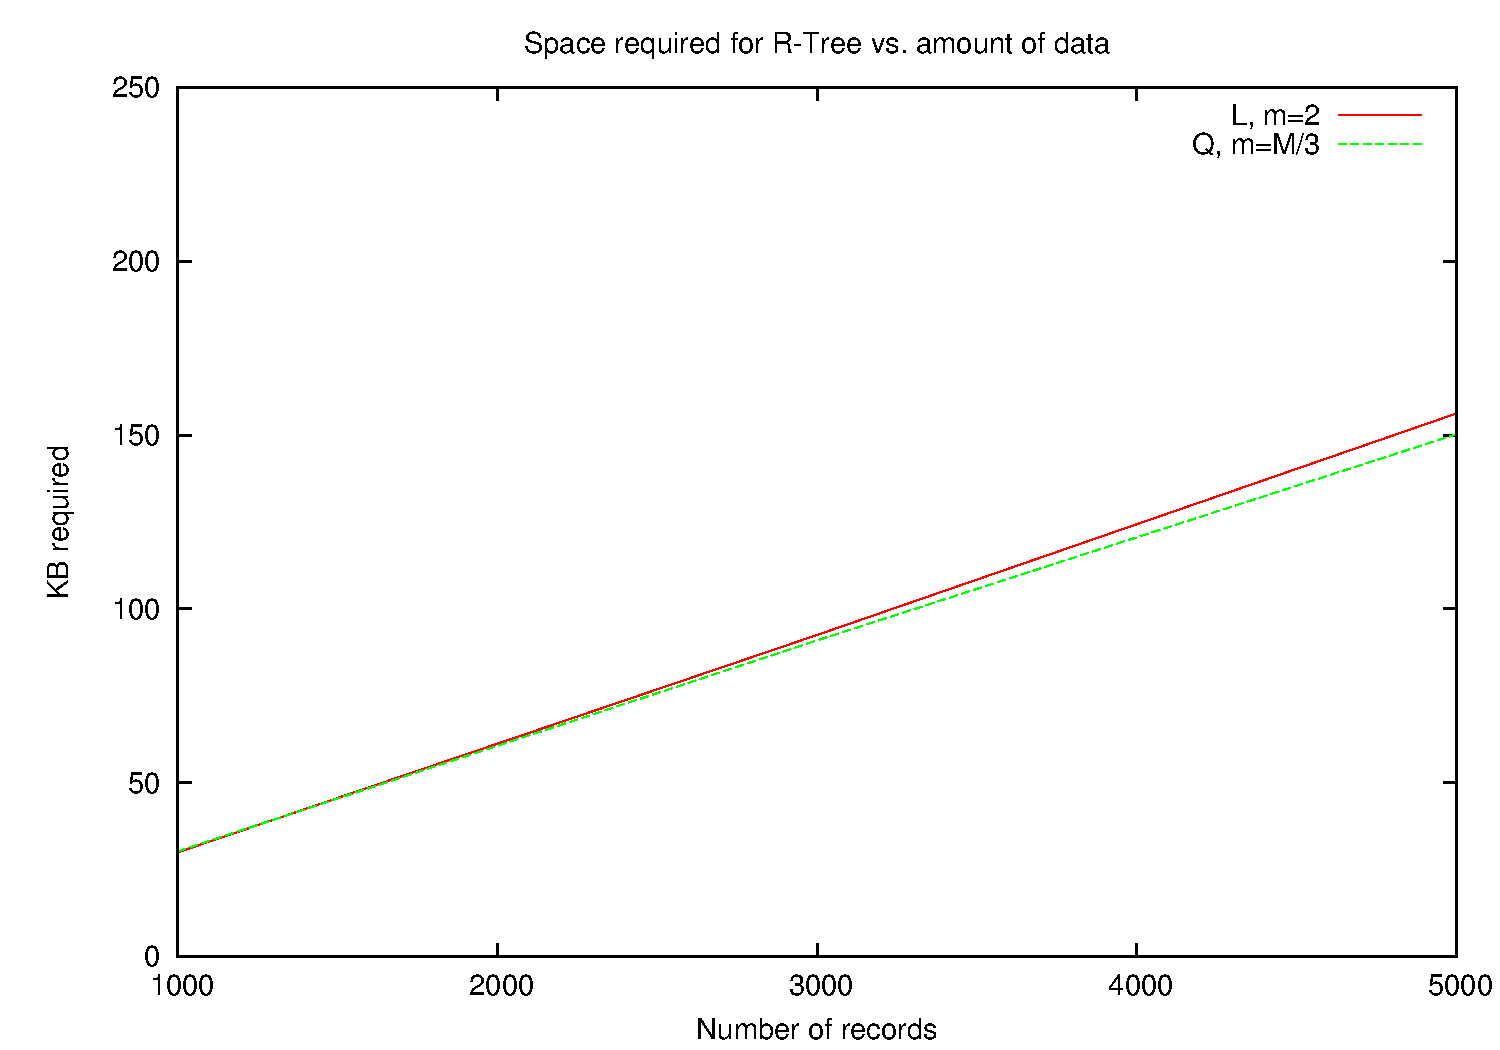
\includegraphics[width=\textwidth]{fig/random/figure-4-10.pdf}
\end{minipage}
\begin{minipage}{0.49\textwidth}
\centering
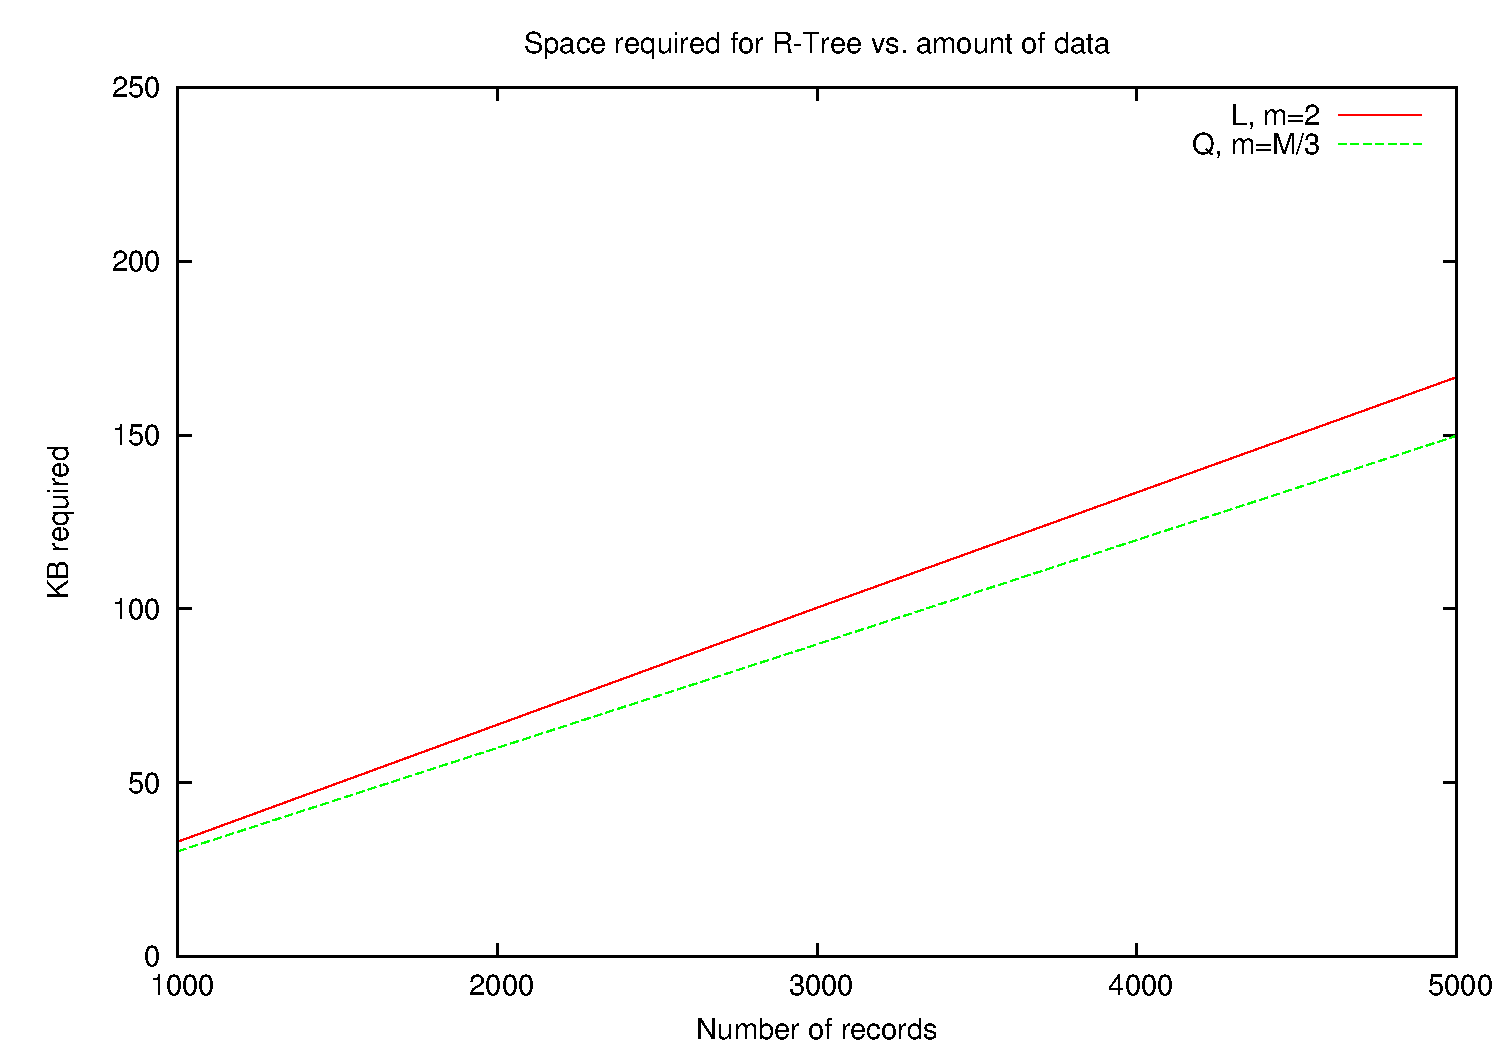
\includegraphics[width=\textwidth]{fig/usppp/figure-4-10.pdf}
\end{minipage}
\caption{Space required for R-Tree vs amount of data}
\label{fig:4.10}
\end{figure}

Figure~\ref{fig:4.10} supports the last hypothesis that space consumption increases linearly with the number of tree entries. 



%====== DISCUSSION ==================
\section{Conclusion}
\label{sec:discussion}
Even after almost 30 years, many of the original R-Tree paper's hypotheses still hold true today. The ones we were not able to empirically support, even though mathematically they make sense, are those concerning significant insert/delete operation differences between linear and quadratic algorithms, search performance over different numbers of records. The former is most likely due to implementation differences and significant improvements in computer hardware: at small scale quadratic vs. linear runtime does not matter as much anymore. The latter, as explained in the previous section, may be due to a flaw in the experimental description in the original paper. Overall, we observed very little difference between the two very different data sets we tested.


\bibliographystyle{abbrv}
\bibliography{main}

\end{document}